\documentclass{book}
\usepackage[a4paper,top=2.5cm,bottom=2.5cm,left=2.5cm,right=2.5cm]{geometry}
\usepackage{makeidx}
\usepackage{natbib}
\usepackage{graphicx}
\usepackage{multicol}
\usepackage{float}
\usepackage{listings}
\usepackage{color}
\usepackage{ifthen}
\usepackage[table]{xcolor}
\usepackage{textcomp}
\usepackage{alltt}
\usepackage{ifpdf}
\ifpdf
\usepackage[pdftex,
            pagebackref=true,
            colorlinks=true,
            linkcolor=blue,
            unicode
           ]{hyperref}
\else
\usepackage[ps2pdf,
            pagebackref=true,
            colorlinks=true,
            linkcolor=blue,
            unicode
           ]{hyperref}
\usepackage{pspicture}
\fi
\usepackage[utf8]{inputenc}
\usepackage{mathptmx}
\usepackage[scaled=.90]{helvet}
\usepackage{courier}
\usepackage{sectsty}
\usepackage{amssymb}
\usepackage[titles]{tocloft}
\usepackage{doxygen}
\lstset{language=C++,inputencoding=utf8,basicstyle=\footnotesize,breaklines=true,breakatwhitespace=true,tabsize=4,numbers=left }
\makeindex
\setcounter{tocdepth}{3}
\renewcommand{\footrulewidth}{0.4pt}
\renewcommand{\familydefault}{\sfdefault}
\hfuzz=15pt
\setlength{\emergencystretch}{15pt}
\hbadness=750
\tolerance=750
\begin{document}
\hypersetup{pageanchor=false,citecolor=blue}
\begin{titlepage}
\vspace*{7cm}
\begin{center}
{\Large Parallel Molecular Dynamics with a Time-\/\-Reversible Nose-\/\-Hoover Thermostat on C\-P\-Us and G\-P\-Us \\[1ex]\large 1.\-0 }\\
\vspace*{1cm}
{\large Generated by Doxygen 1.8.2}\\
\vspace*{0.5cm}
{\small Sun Jan 12 2014 14:56:52}\\
\end{center}
\end{titlepage}
\clearemptydoublepage
\pagenumbering{roman}
\tableofcontents
\clearemptydoublepage
\pagenumbering{arabic}
\hypersetup{pageanchor=true,citecolor=blue}
\chapter{C\-B\-E\-M\-D\-G\-P\-U}
\label{md_README}
\hypertarget{md_README}{}
\begin{quotation}
C\-B\-E M\-D on G\-P\-Us

\end{quotation}


\begin{quotation}
\begin{quotation}
by Nathan A. Mahynski, George A. Khoury, and Carmeline J. Dsilva

\end{quotation}


\end{quotation}


See \hyperlink{main_8cpp_source}{main.\-cpp} to set parameters which are documented by example in this file.

To compile the C\-P\-U version, type \$ make M\-D

To compile the G\-P\-U version, type \$ make -\/f Makefile\-\_\-cuda

To compile tests, type \$ make T\-E\-S\-T\-S

To compile the timing executable (used for scaling studies), type \$ make T\-I\-M\-I\-N\-G

To compile the program that runs a simulation to compare with L\-A\-M\-M\-P\-S output, type \$ make L\-M\-P\-\_\-\-C\-O\-M\-P\-A\-R\-E

To compile the program that tests the N\-V\-E integrator, type \$ make T\-E\-S\-T\-\_\-\-N\-V\-E

In the Makefile, the P\-A\-T\-H\-T\-O\-B\-O\-O\-S\-T variable should point to the diretory where the C++ boost libraries are saved.

In the G\-T\-E\-S\-T\-\_\-\-D\-I\-R variable should point to the directory where the Google Tests libraries are saved.

Note that the Intel C++ compilers must be used; the G\-N\-U C++ compilers do not work with the Open\-M\-P portion of our code (this is a known bug in the compiler, see F\-Y\-I section).

\section*{Execution}

\hyperlink{main_8cpp_source}{main.\-cpp} expects 4 input, the number of threads to use with O\-M\-P, the number of atoms, the skin radius for the cell/neighbor lists, and the number of steps to simulate. \$ ./md $<$nthreads$>$ $<$natoms$>$ $<$rs$>$ $<$nsteps$>$ $>$ log 2$>$ err

This also produces a trajectory.\-xyz file which can be visualized with V\-M\-D (if you have it installed) \$ vmd -\/xyz trajectory.\-xyz

\section*{Explanation of \hyperlink{main_8cpp_source}{main.\-cpp}}

\begin{quotation}
How to use, change, and make your own in 10 steps.

\end{quotation}



\begin{DoxyEnumerate}
\item \hyperlink{main_8cpp_source}{main.\-cpp} expects 4 input, the number of threads to use with O\-M\-P, the number of atoms, the skin radius for the cell/neighbor lists, and the number of steps to simulate. \$ ./md $<$nthreads$>$ $<$natoms$>$ $<$rs$>$ $<$nsteps$>$ $>$ log 2$>$ err
\end{DoxyEnumerate}


\begin{DoxyEnumerate}
\item The random number generator seed is then set manually to ensure that results are reproducible.
\end{DoxyEnumerate}


\begin{DoxyEnumerate}
\item The user must then specify basic properties about the system. A \hyperlink{classsystem_definition}{system\-Definition} object should be instantiated and then temperature, box size, particle mass, and pair potential cutoff should be specified

\$ \hyperlink{classsystem_definition}{system\-Definition} a;

\$ a.\-set\-Temp(1.\-0);...
\end{DoxyEnumerate}


\begin{DoxyEnumerate}
\item The system can then be initialized with the command init\-Thermal or init\-Random (see doxygen documentation for more details). For example, in the former\-:

\$ a.\-init\-Thermal(n\-Atoms, Temp, rng\-Seed, separation);
\end{DoxyEnumerate}


\begin{DoxyEnumerate}
\item Where \char`\"{}n\-Atoms\char`\"{} is the number of atoms, \char`\"{}separation\char`\"{} is the initial separation of the particles on the simple cubic lattice on which they are initialized, and the rest of the variables are self-\/explanatory. This command completely initializes the system for simulation.
\end{DoxyEnumerate}


\begin{DoxyEnumerate}
\item Next, the pair potential should be specified. As an example in \hyperlink{main_8cpp_source}{main.\-cpp}, the preprocessor flag N\-V\-C\-C is used to select either the C\-P\-U version of the shifted lennard-\/jones potential (slj) or the G\-P\-U version (dev\-\_\-slj). The Makefile (compare to Makefile\-\_\-cuda) will define this if necessary and allows the code to flow naturally and work in both cases.

\$ point\-Function\-\_\-t pp = slj;

\$ a.\-set\-Potential(pp);
\end{DoxyEnumerate}


\begin{DoxyEnumerate}
\item If the G\-P\-Us are used (N\-V\-C\-C compiler flag is defined) the number of threads and blocks the G\-P\-U kernel will be invoked with must be set. This is done next.
\end{DoxyEnumerate}


\begin{DoxyEnumerate}
\item Then additional arguments for the pair potential must be specified. In the case of the slj function, variables epsilon, sigma, delta, and ushift must be given. This is then set in the \hyperlink{classsystem_definition}{system\-Definition}.

\$ std\-::vector $<$float$>$ args(5);

\$ args\mbox{[}0\mbox{]} = 1.\-0; // epsilon

\$ args\mbox{[}1\mbox{]} = 1.\-0; // sigma

\$ args\mbox{[}2\mbox{]} = 0.\-0; // delta

\$ args\mbox{[}3\mbox{]} = 0.\-0; // ushift

\$ a.\-set\-Potential\-Args(args);
\end{DoxyEnumerate}


\begin{DoxyEnumerate}
\item Afterwards, the integrator (ensemble) must be specified. In the case of the N\-V\-T ensemble where we are using the Nose-\/\-Hoover thermostat, the integrator is given by the object \hyperlink{classnvt___n_h}{nvt\-\_\-\-N\-H}. This requires a damping constant, which for the slj potential should be about unity. Then the numerical timestep should be given, for the slj this is usually efficient around 0.\-005.

\$ \hyperlink{classnvt___n_h}{nvt\-\_\-\-N\-H} integrate (1.\-0);

\$ integrate.\-set\-Timestep(timestep);
\end{DoxyEnumerate}


\begin{DoxyEnumerate}
\item Finally the simulation is ready to iterate. A simple loop can be set to do this. An example for the case of the N\-V\-E ensemble is also provided in \hyperlink{test__nve_8cpp_source}{test\-\_\-nve.\-cpp} which can be compiled with make T\-E\-S\-T\-\_\-\-N\-V\-E (see \hyperlink{test__nve_8cpp_source}{test\-\_\-nve.\-cpp})
\end{DoxyEnumerate}

\section*{F\-Y\-I}

\begin{quotation}
Known bugs, etc.

\end{quotation}


There are a few known instances of bugs related to compiler options, etc.


\begin{DoxyEnumerate}
\item Using icpc instead of g++ Our code uses O\-M\-P to parallelize many calculations. Specifically, the atoms member (vector) in the \hyperlink{classsystem_definition}{system\-Definition} object must be shared often. However, because it is a member of a class g++ struggles to properly share this in memory. This is a known bug in the g++ compiler which the intel (icpc) version handles rigorously. As a result, our code will produce errors if compiled with the g++ compiler when more than 1 core is used. To use this on tiger the module openmpi/intel-\/12.\-1/1.4.\-5/64 should be loaded to make the icpc compiler accessible.
\end{DoxyEnumerate}


\begin{DoxyEnumerate}
\item Cuda toolkit 5.\-5 C\-U\-D\-A is a finicky tool. Different G\-P\-Us require different toolkits and versions to work properly. In fact, compilation may succeed with a bad version but the run time behavior produces unexpected (incorrect) results. For the K20 cards on tiger, the latest toolkit (v5.\-5) must be loaded. To do so, load the module cudatoolkit/5.\-5.\-22 before attempting to compile the program. The Makefile must include flags consistent with the G\-P\-Us version of C\-U\-D\-A (which on tiger in 3.\-5) so the Makefile\-\_\-cuda contains a flag \char`\"{}\-N\-V\-F\-L\-A\-G\-S = -\/gencode arch=compute\-\_\-35,code=sm\-\_\-35\char`\"{} for the .cu files. Furthermore, you will find that preprocessor flags N\-V\-C\-C and N\-O\-G\-P\-U are found throughout the code which act as switches to activate/deactivate G\-P\-U functionality throughout the compilation process.
\end{DoxyEnumerate}


\begin{DoxyEnumerate}
\item Tiger G\-P\-Us Unfortunately it appears that the queueing system on tiger is having problems reserving all or some of the G\-P\-Us exclusively for single jobs by users. As a result, thrust (the G\-P\-U equivalent of the S\-T\-L for C++) will have memory issues if one or more of the G\-P\-Us on a node are already in use. Because of the unusually high load on tiger over the past month, we have been unable to obtain good results on this cluster since usually this situation is encountered. Our private G\-P\-U cluster was used to obtian our results instead, though our Makefile\-\_\-cuda is set so this should compile properly on tiger if you want to check. 
\end{DoxyEnumerate}
\chapter{Hierarchical Index}
\section{Class Hierarchy}
This inheritance list is sorted roughly, but not completely, alphabetically\-:\begin{DoxyCompactList}
\item \contentsline{section}{atom}{\pageref{structatom}}{}
\item \contentsline{section}{cell\-List\-\_\-cpu}{\pageref{classcell_list__cpu}}{}
\item exception\begin{DoxyCompactList}
\item \contentsline{section}{custom\-Exception}{\pageref{classcustom_exception}}{}
\end{DoxyCompactList}
\item \contentsline{section}{float3}{\pageref{structfloat3}}{}
\item \contentsline{section}{int3}{\pageref{structint3}}{}
\item \contentsline{section}{integrator}{\pageref{classintegrator}}{}
\begin{DoxyCompactList}
\item \contentsline{section}{nve}{\pageref{classnve}}{}
\item \contentsline{section}{nvt\-\_\-\-N\-H}{\pageref{classnvt___n_h}}{}
\end{DoxyCompactList}
\item \contentsline{section}{system\-Definition}{\pageref{classsystem_definition}}{}
\item \contentsline{section}{system\-Props}{\pageref{classsystem_props}}{}
\item Test\begin{DoxyCompactList}
\item \contentsline{section}{System\-Test}{\pageref{class_system_test}}{}
\end{DoxyCompactList}
\end{DoxyCompactList}

\chapter{Class Index}
\section{Class List}
Here are the classes, structs, unions and interfaces with brief descriptions\-:\begin{DoxyCompactList}
\item\contentsline{section}{\hyperlink{structatom}{atom} \\*Structure of an atom }{\pageref{structatom}}{}
\item\contentsline{section}{\hyperlink{classcell_list__cpu}{cell\-List\-\_\-cpu} }{\pageref{classcell_list__cpu}}{}
\item\contentsline{section}{\hyperlink{classcustom_exception}{custom\-Exception} \\*Error reporting }{\pageref{classcustom_exception}}{}
\item\contentsline{section}{\hyperlink{structfloat3}{float3} \\*3 floating point numbers, same as defined for G\-P\-Us }{\pageref{structfloat3}}{}
\item\contentsline{section}{\hyperlink{structint3}{int3} \\*3 integers, same as defined for G\-P\-Us }{\pageref{structint3}}{}
\item\contentsline{section}{\hyperlink{classintegrator}{integrator} \\*Base class for integrators such as N\-V\-T (Nose-\/\-Hoover) or N\-V\-E ensembles }{\pageref{classintegrator}}{}
\item\contentsline{section}{\hyperlink{classnve}{nve} \\*Integration scheme that preserves total energy of the system }{\pageref{classnve}}{}
\item\contentsline{section}{\hyperlink{classnvt___n_h}{nvt\-\_\-\-N\-H} \\*Uses Nose-\/\-Hover integration method to thermostat a system (constant T rather than E) }{\pageref{classnvt___n_h}}{}
\item\contentsline{section}{\hyperlink{classsystem_definition}{system\-Definition} \\*Contains all information pertaining to a system being simulated }{\pageref{classsystem_definition}}{}
\item\contentsline{section}{\hyperlink{classsystem_props}{system\-Props} \\*Holds all information about the C\-P\-U and G\-P\-U the simulation is being performed on }{\pageref{classsystem_props}}{}
\item\contentsline{section}{\hyperlink{class_system_test}{System\-Test} }{\pageref{class_system_test}}{}
\end{DoxyCompactList}

\chapter{Class Documentation}
\hypertarget{structatom}{\section{atom Struct Reference}
\label{structatom}\index{atom@{atom}}
}


Structure of an atom.  




{\ttfamily \#include $<$data\-Types.\-h$>$}

\subsection*{Public Attributes}
\begin{DoxyCompactItemize}
\item 
\hypertarget{structatom_a6f304469ecac52a860f325ae6ac9ca34}{\hyperlink{structfloat3}{float3} \hyperlink{structatom_a6f304469ecac52a860f325ae6ac9ca34}{pos}}\label{structatom_a6f304469ecac52a860f325ae6ac9ca34}

\begin{DoxyCompactList}\small\item\em Position. \end{DoxyCompactList}\item 
\hypertarget{structatom_a010b2c50c7cdb6e4ec796e0c369e84d9}{\hyperlink{structfloat3}{float3} \hyperlink{structatom_a010b2c50c7cdb6e4ec796e0c369e84d9}{vel}}\label{structatom_a010b2c50c7cdb6e4ec796e0c369e84d9}

\begin{DoxyCompactList}\small\item\em Velocity. \end{DoxyCompactList}\item 
\hypertarget{structatom_a0d0e70ef3922064b59b805ac0f81d460}{\hyperlink{structfloat3}{float3} \hyperlink{structatom_a0d0e70ef3922064b59b805ac0f81d460}{acc}}\label{structatom_a0d0e70ef3922064b59b805ac0f81d460}

\begin{DoxyCompactList}\small\item\em Acceleration. \end{DoxyCompactList}\end{DoxyCompactItemize}


\subsection{Detailed Description}
Structure of an atom. 

Definition at line 29 of file data\-Types.\-h.



The documentation for this struct was generated from the following file\-:\begin{DoxyCompactItemize}
\item 
/\-Users/nathanmahynski/\-Desktop/\-C\-B\-E\-M\-D\-G\-P\-U/data\-Types.\-h\end{DoxyCompactItemize}

\hypertarget{classcell_list__cpu}{\section{cell\-List\-\_\-cpu Class Reference}
\label{classcell_list__cpu}\index{cell\-List\-\_\-cpu@{cell\-List\-\_\-cpu}}
}


{\ttfamily \#include $<$cell\-List.\-h$>$}

\subsection*{Public Member Functions}
\begin{DoxyCompactItemize}
\item 
\hyperlink{classcell_list__cpu_a2ac134374c8e561617433e03bb6b2d1e}{cell\-List\-\_\-cpu} (const \hyperlink{structfloat3}{float3} \&box, const float rc, const float rs)
\item 
void \hyperlink{classcell_list__cpu_a70568e6a2012eb8592f2798b3260c550}{check\-Update} (const \hyperlink{classsystem_definition}{system\-Definition} \&sys)
\begin{DoxyCompactList}\small\item\em Check if the neighbor list requires updating. \end{DoxyCompactList}\item 
int \hyperlink{classcell_list__cpu_a564d95c9bd7af0829291789d173361e0}{cell} (const \hyperlink{structfloat3}{float3} \&pos)
\begin{DoxyCompactList}\small\item\em Calculate the cell in which a given coordinate is located. \end{DoxyCompactList}\item 
\hypertarget{classcell_list__cpu_a0769d2a8a9c6964a8c6894bab9841e71}{int \hyperlink{classcell_list__cpu_a0769d2a8a9c6964a8c6894bab9841e71}{head} (const int \hyperlink{classcell_list__cpu_a564d95c9bd7af0829291789d173361e0}{cell}) const }\label{classcell_list__cpu_a0769d2a8a9c6964a8c6894bab9841e71}

\begin{DoxyCompactList}\small\item\em Return the first atom (aka 'head') of each cell. \end{DoxyCompactList}\item 
\hypertarget{classcell_list__cpu_ac274503e6cc75811e9cb9c07120fb96e}{int \hyperlink{classcell_list__cpu_ac274503e6cc75811e9cb9c07120fb96e}{list} (const int index) const }\label{classcell_list__cpu_ac274503e6cc75811e9cb9c07120fb96e}

\begin{DoxyCompactList}\small\item\em Iterates through a linked list of particles, returns the index of the next atom in line. \end{DoxyCompactList}\item 
\hypertarget{classcell_list__cpu_aeaf165c887b13bfa7f7c1a8b70102aff}{std\-::vector$<$ int $>$ \hyperlink{classcell_list__cpu_aeaf165c887b13bfa7f7c1a8b70102aff}{neighbors} (const int cell\-I\-D) const }\label{classcell_list__cpu_aeaf165c887b13bfa7f7c1a8b70102aff}

\begin{DoxyCompactList}\small\item\em Returns the indices of a cell's neighboring cells. \end{DoxyCompactList}\end{DoxyCompactItemize}
\subsection*{Public Attributes}
\begin{DoxyCompactItemize}
\item 
\hypertarget{classcell_list__cpu_ae86e1c9604a39bc8a493fa0f6538fd37}{\hyperlink{structint3}{int3} \hyperlink{classcell_list__cpu_ae86e1c9604a39bc8a493fa0f6538fd37}{n\-Cells}}\label{classcell_list__cpu_ae86e1c9604a39bc8a493fa0f6538fd37}

\begin{DoxyCompactList}\small\item\em Number of cells in each direction. \end{DoxyCompactList}\end{DoxyCompactItemize}


\subsection{Detailed Description}
Cell Lists \begin{DoxyAuthor}{Author}
Nathan A. Mahynski 
\end{DoxyAuthor}
\begin{DoxyDate}{Date}
11/19/13
\end{DoxyDate}
Maintains a linked list to track cells on the C\-P\-U 

Definition at line 39 of file cell\-List.\-h.



\subsection{Constructor \& Destructor Documentation}
\hypertarget{classcell_list__cpu_a2ac134374c8e561617433e03bb6b2d1e}{\index{cell\-List\-\_\-cpu@{cell\-List\-\_\-cpu}!cell\-List\-\_\-cpu@{cell\-List\-\_\-cpu}}
\index{cell\-List\-\_\-cpu@{cell\-List\-\_\-cpu}!cellList_cpu@{cell\-List\-\_\-cpu}}
\subsubsection[{cell\-List\-\_\-cpu}]{\setlength{\rightskip}{0pt plus 5cm}cell\-List\-\_\-cpu\-::cell\-List\-\_\-cpu (
\begin{DoxyParamCaption}
\item[{const {\bf float3} \&}]{box, }
\item[{const float}]{rc, }
\item[{const float}]{rs}
\end{DoxyParamCaption}
)}}\label{classcell_list__cpu_a2ac134374c8e561617433e03bb6b2d1e}
Cell Lists \begin{DoxyAuthor}{Author}
Nathan A. Mahynski 
\end{DoxyAuthor}
\begin{DoxyDate}{Date}
11/19/13
\end{DoxyDate}
Initialize a cell list


\begin{DoxyParams}[1]{Parameters}
\mbox{\tt in}  & {\em box} & Box size \\
\hline
\mbox{\tt in}  & {\em rc} & Cutoff radius \\
\hline
\mbox{\tt in}  & {\em rs} & Skin Radius \\
\hline
\end{DoxyParams}


Definition at line 156 of file cell\-List.\-cpp.



References n\-Cells.


\begin{DoxyCode}
                                                                             \{
    \textcolor{keywordflow}{if} (rc < 0.0) \{
    \textcolor{keywordflow}{throw} \hyperlink{classcustom_exception}{customException}(\textcolor{stringliteral}{"Cutoff radius must be > 0"});
    \textcolor{keywordflow}{return};
    \}
    rc\_ = rc;
    \textcolor{keywordflow}{if} (rs < 0.0) \{
    \textcolor{keywordflow}{throw} \hyperlink{classcustom_exception}{customException}(\textcolor{stringliteral}{"Skin radius must be > 0"});
    \textcolor{keywordflow}{return};
    \}
    rs\_ = rs;

    box\_ = box;

    start\_ = 1;
    lcell\_.x = 1.01*(rc+rs);
    \hyperlink{classcell_list__cpu_ae86e1c9604a39bc8a493fa0f6538fd37}{nCells}.x = (int) floor (box.x/lcell\_.x);
    lcell\_.x = (box.x/\hyperlink{classcell_list__cpu_ae86e1c9604a39bc8a493fa0f6538fd37}{nCells}.x);

    lcell\_.y = 1.01*(rc+rs);
    \hyperlink{classcell_list__cpu_ae86e1c9604a39bc8a493fa0f6538fd37}{nCells}.y = (int) floor (box.y/lcell\_.y);
    lcell\_.y = (box.y/\hyperlink{classcell_list__cpu_ae86e1c9604a39bc8a493fa0f6538fd37}{nCells}.y);

    lcell\_.z = 1.01*(rc+rs);
    \hyperlink{classcell_list__cpu_ae86e1c9604a39bc8a493fa0f6538fd37}{nCells}.z = (int) floor (box.z/lcell\_.z);
    lcell\_.z = (box.z/\hyperlink{classcell_list__cpu_ae86e1c9604a39bc8a493fa0f6538fd37}{nCells}.z);

    \textcolor{keywordflow}{if} (lcell\_.x <= (rc+rs) || lcell\_.y <= (rc+rs) || lcell\_.z < (rc+rs)) \{
    \textcolor{keywordflow}{throw} \hyperlink{classcustom_exception}{customException}(\textcolor{stringliteral}{"Cell width must exceed sum of cutoff
       and skin radius"});
    \textcolor{keywordflow}{return};
    \}

    \textcolor{keywordflow}{if} (lcell\_.x < 1) \{
    \textcolor{keywordflow}{throw} \hyperlink{classcustom_exception}{customException} (\textcolor{stringliteral}{"Box dimension x too small relative
       to skin and cutoff radius to use cell lists"});
    \textcolor{keywordflow}{return};
    \}
    \textcolor{keywordflow}{if} (lcell\_.y < 1) \{
    \textcolor{keywordflow}{throw} \hyperlink{classcustom_exception}{customException} (\textcolor{stringliteral}{"Box dimension y too small relative
       to skin and cutoff radius to use cell lists"});
    \textcolor{keywordflow}{return};
    \}
    \textcolor{keywordflow}{if} (lcell\_.z < 1) \{
    \textcolor{keywordflow}{throw} \hyperlink{classcustom_exception}{customException} (\textcolor{stringliteral}{"Box dimension z too small relative
       to skin and cutoff radius to use cell lists"});
    \textcolor{keywordflow}{return};
    \}

    \textcolor{keywordflow}{if} (\hyperlink{classcell_list__cpu_ae86e1c9604a39bc8a493fa0f6538fd37}{nCells}.x < 3 || \hyperlink{classcell_list__cpu_ae86e1c9604a39bc8a493fa0f6538fd37}{nCells}.y < 3 || \hyperlink{classcell_list__cpu_ae86e1c9604a39bc8a493fa0f6538fd37}{nCells}.z < 3) \{
    \textcolor{keywordflow}{throw} \hyperlink{classcustom_exception}{customException}(\textcolor{stringliteral}{"Must be able to have at least 3 cells
       in each direction, change box size, skin, or cutoff radius"});
    \textcolor{keywordflow}{return};
    \}

    \textcolor{keywordflow}{try} \{
    head\_.resize(\hyperlink{classcell_list__cpu_ae86e1c9604a39bc8a493fa0f6538fd37}{nCells}.x*\hyperlink{classcell_list__cpu_ae86e1c9604a39bc8a493fa0f6538fd37}{nCells}.y*\hyperlink{classcell_list__cpu_ae86e1c9604a39bc8a493fa0f6538fd37}{nCells}.z, -1);
    \} \textcolor{keywordflow}{catch} (std::exception &e) \{
    std::cerr << e.what() << std::endl;
    \textcolor{keywordflow}{throw} \hyperlink{classcustom_exception}{customException} (\textcolor{stringliteral}{"Unable to initialize head for cell
       list"});
    \textcolor{keywordflow}{return};
    \}
    \textcolor{comment}{// build neighbors for each cell}
    neighbor\_.resize(\hyperlink{classcell_list__cpu_ae86e1c9604a39bc8a493fa0f6538fd37}{nCells}.x*\hyperlink{classcell_list__cpu_ae86e1c9604a39bc8a493fa0f6538fd37}{nCells}.y*\hyperlink{classcell_list__cpu_ae86e1c9604a39bc8a493fa0f6538fd37}{nCells}.z);
    \textcolor{keywordflow}{for} (\textcolor{keywordtype}{unsigned} \textcolor{keywordtype}{int} cellID = 0; cellID < \hyperlink{classcell_list__cpu_ae86e1c9604a39bc8a493fa0f6538fd37}{nCells}.x*\hyperlink{classcell_list__cpu_ae86e1c9604a39bc8a493fa0f6538fd37}{nCells}.y*\hyperlink{classcell_list__cpu_ae86e1c9604a39bc8a493fa0f6538fd37}{nCells}
      .z; ++cellID) \{
        \textcolor{keyword}{const} \textcolor{keywordtype}{int} zref = floor(cellID/(\hyperlink{classcell_list__cpu_ae86e1c9604a39bc8a493fa0f6538fd37}{nCells}.x*\hyperlink{classcell_list__cpu_ae86e1c9604a39bc8a493fa0f6538fd37}{nCells}.y));
        \textcolor{keyword}{const} \textcolor{keywordtype}{int} yref = floor((cellID - zref*(\hyperlink{classcell_list__cpu_ae86e1c9604a39bc8a493fa0f6538fd37}{nCells}.x*\hyperlink{classcell_list__cpu_ae86e1c9604a39bc8a493fa0f6538fd37}{nCells}.y))/
      \hyperlink{classcell_list__cpu_ae86e1c9604a39bc8a493fa0f6538fd37}{nCells}.y);
        \textcolor{keyword}{const} \textcolor{keywordtype}{int} xref = floor(cellID - zref*(\hyperlink{classcell_list__cpu_ae86e1c9604a39bc8a493fa0f6538fd37}{nCells}.x*\hyperlink{classcell_list__cpu_ae86e1c9604a39bc8a493fa0f6538fd37}{nCells}.y) - 
      yref*\hyperlink{classcell_list__cpu_ae86e1c9604a39bc8a493fa0f6538fd37}{nCells}.x);
        \textcolor{keywordflow}{for} (\textcolor{keywordtype}{int} dx = -1; dx <= 1; ++dx) \{
        \textcolor{keywordtype}{int} xcell = xref + dx;
        \textcolor{keywordflow}{if} (xcell >= \hyperlink{classcell_list__cpu_ae86e1c9604a39bc8a493fa0f6538fd37}{nCells}.x) xcell = 0;
        \textcolor{keywordflow}{if} (xcell < 0) xcell = \hyperlink{classcell_list__cpu_ae86e1c9604a39bc8a493fa0f6538fd37}{nCells}.x-1;
        \textcolor{keywordflow}{for} (\textcolor{keywordtype}{int} dy = -1; dy <= 1; ++dy) \{
            \textcolor{keywordtype}{int} ycell = yref + dy;
            \textcolor{keywordflow}{if} (ycell >= \hyperlink{classcell_list__cpu_ae86e1c9604a39bc8a493fa0f6538fd37}{nCells}.y) ycell = 0;
            \textcolor{keywordflow}{if} (ycell < 0) ycell = \hyperlink{classcell_list__cpu_ae86e1c9604a39bc8a493fa0f6538fd37}{nCells}.y-1;
            \textcolor{keywordflow}{for} (\textcolor{keywordtype}{int} dz = -1; dz <= 1; ++dz) \{
            \textcolor{keywordtype}{int} zcell = zref + dz;
            \textcolor{keywordflow}{if} (zcell >= \hyperlink{classcell_list__cpu_ae86e1c9604a39bc8a493fa0f6538fd37}{nCells}.z) zcell = 0;
            \textcolor{keywordflow}{if} (zcell < 0) zcell = \hyperlink{classcell_list__cpu_ae86e1c9604a39bc8a493fa0f6538fd37}{nCells}.z-1;
            \textcolor{keyword}{const} \textcolor{keywordtype}{int} cellID2 = xcell + ycell*\hyperlink{classcell_list__cpu_ae86e1c9604a39bc8a493fa0f6538fd37}{nCells}.x + zcell*(\hyperlink{classcell_list__cpu_ae86e1c9604a39bc8a493fa0f6538fd37}{nCells}
      .x*\hyperlink{classcell_list__cpu_ae86e1c9604a39bc8a493fa0f6538fd37}{nCells}.y);
            neighbor\_[cellID].push\_back(cellID2);
            \}
        \}
        \}
    \}
    \textcolor{keywordflow}{for} (\textcolor{keywordtype}{unsigned} \textcolor{keywordtype}{int} cellID = 0; cellID < \hyperlink{classcell_list__cpu_ae86e1c9604a39bc8a493fa0f6538fd37}{nCells}.x*\hyperlink{classcell_list__cpu_ae86e1c9604a39bc8a493fa0f6538fd37}{nCells}.y*\hyperlink{classcell_list__cpu_ae86e1c9604a39bc8a493fa0f6538fd37}{nCells}
      .z; ++cellID) \{
    \textcolor{keywordflow}{if} (neighbor\_[cellID].size() != 27) \{
        \textcolor{keywordflow}{throw} \hyperlink{classcustom_exception}{customException} (\textcolor{stringliteral}{"Cell list initial build failed
       to find 27 neighbors (including self)"});
        \textcolor{keywordflow}{return};
    \}
    \}
\}
\end{DoxyCode}


\subsection{Member Function Documentation}
\hypertarget{classcell_list__cpu_a564d95c9bd7af0829291789d173361e0}{\index{cell\-List\-\_\-cpu@{cell\-List\-\_\-cpu}!cell@{cell}}
\index{cell@{cell}!cellList_cpu@{cell\-List\-\_\-cpu}}
\subsubsection[{cell}]{\setlength{\rightskip}{0pt plus 5cm}int cell\-List\-\_\-cpu\-::cell (
\begin{DoxyParamCaption}
\item[{const {\bf float3} \&}]{pos}
\end{DoxyParamCaption}
)}}\label{classcell_list__cpu_a564d95c9bd7af0829291789d173361e0}


Calculate the cell in which a given coordinate is located. 

Calculates the cell (linear index of it) a position belongs to in a periodic box. The position does not need to be \char`\"{}inside\char`\"{} the box, boundary conditions are applied.


\begin{DoxyParams}[1]{Parameters}
\mbox{\tt in}  & {\em pos} & Position of atom \\
\hline
\end{DoxyParams}
\begin{DoxyReturn}{Returns}
cell 
\end{DoxyReturn}


Definition at line 252 of file cell\-List.\-cpp.



References n\-Cells.



Referenced by check\-Update(), and head().


\begin{DoxyCode}
                                         \{
    \hyperlink{structfloat3}{float3} inBox = pbc(pos, box\_);
    \textcolor{keyword}{const} \textcolor{keywordtype}{int} x = (int) floor(inBox.x/lcell\_.x);
    \textcolor{keyword}{const} \textcolor{keywordtype}{int} y = (int) floor(inBox.y/lcell\_.y);
    \textcolor{keyword}{const} \textcolor{keywordtype}{int} z = (int) floor(inBox.z/lcell\_.z);
    \textcolor{keywordflow}{return} x + y*\hyperlink{classcell_list__cpu_ae86e1c9604a39bc8a493fa0f6538fd37}{nCells}.x + z*\hyperlink{classcell_list__cpu_ae86e1c9604a39bc8a493fa0f6538fd37}{nCells}.x*\hyperlink{classcell_list__cpu_ae86e1c9604a39bc8a493fa0f6538fd37}{nCells}.y;
\}
\end{DoxyCode}
\hypertarget{classcell_list__cpu_a70568e6a2012eb8592f2798b3260c550}{\index{cell\-List\-\_\-cpu@{cell\-List\-\_\-cpu}!check\-Update@{check\-Update}}
\index{check\-Update@{check\-Update}!cellList_cpu@{cell\-List\-\_\-cpu}}
\subsubsection[{check\-Update}]{\setlength{\rightskip}{0pt plus 5cm}void cell\-List\-\_\-cpu\-::check\-Update (
\begin{DoxyParamCaption}
\item[{const {\bf system\-Definition} \&}]{sys}
\end{DoxyParamCaption}
)}}\label{classcell_list__cpu_a70568e6a2012eb8592f2798b3260c550}


Check if the neighbor list requires updating. 

Checks to see if the cell list needs to be updated and if so, rebuilds Uses linked list, so algorithm in O(\-N)


\begin{DoxyParams}[1]{Parameters}
\mbox{\tt in}  & {\em sys} & System definition \\
\hline
\end{DoxyParams}


Definition at line 266 of file cell\-List.\-cpp.



References system\-Definition\-::atoms, system\-Definition\-::box(), cell(), and system\-Definition\-::num\-Atoms().



Referenced by integrator\-::calc\-Force().


\begin{DoxyCode}
                                                           \{
    \textcolor{keywordtype}{int} build = 0;
    \textcolor{keywordflow}{if} (start\_) \{
    \textcolor{keyword}{const} \textcolor{keywordtype}{int} natoms = sys.\hyperlink{classsystem_definition_ae8d3c2df2d56241cee03fcc4e2026ae0}{numAtoms}();
    \textcolor{keywordflow}{try} \{
            list\_.resize(natoms, -1);
        \} \textcolor{keywordflow}{catch} (std::exception& e) \{
            std::cerr << e.what() << std::endl;
            \textcolor{keywordflow}{throw} \hyperlink{classcustom_exception}{customException} (\textcolor{stringliteral}{"Unable to initialize list
       for cell list"});
            \textcolor{keywordflow}{return};
        \}
        \textcolor{keywordflow}{try} \{
            posAtLastBuild\_.resize(natoms);
        \} \textcolor{keywordflow}{catch} (std::exception& e) \{
            std::cerr << e.what() << std::endl;
            \textcolor{keywordflow}{throw} \hyperlink{classcustom_exception}{customException} (\textcolor{stringliteral}{"Unable to initialize
       position list for cell list"});
            \textcolor{keywordflow}{return};
        \}
        start\_ = 0;
        build = 1;
    \} \textcolor{keywordflow}{else} \{
        \textcolor{comment}{// check max displacements}
        \textcolor{keywordtype}{float} drMax1\_ = 0.0;
        \textcolor{keywordtype}{float} drMax2\_ = 0.0;
        \hyperlink{structfloat3}{float3} dummy;
            \textcolor{keywordflow}{for} (\textcolor{keywordtype}{unsigned} \textcolor{keywordtype}{int} i = 0; i < sys.\hyperlink{classsystem_definition_ae8d3c2df2d56241cee03fcc4e2026ae0}{numAtoms}(); ++i) \{
                \textcolor{keyword}{const} \textcolor{keywordtype}{float} dr2 = pbcDist2 (sys.\hyperlink{classsystem_definition_ae8814d3f60fc1111af2a3f218a4bfcab}{atoms}[i].pos, 
      posAtLastBuild\_[i], dummy, sys.\hyperlink{classsystem_definition_a85b80dee3609ddb68e370cee3fa959ea}{box}());
                \textcolor{keywordflow}{if} (dr2 > drMax1\_*drMax1\_) \{
                    drMax2\_ = drMax1\_;
                    drMax1\_ = sqrt(dr2);
                \} \textcolor{keywordflow}{else} \textcolor{keywordflow}{if} (dr2 > drMax2\_*drMax2\_) \{
                    drMax2\_ = sqrt(dr2);
                \}
            \}
        \textcolor{keywordflow}{if} (drMax1\_+drMax2\_ > rs\_) \{
            build = 1;
        \} \textcolor{keywordflow}{else} \{
            build = 0;
        \}
    \}

    \textcolor{keywordflow}{if} (build) \{
        \textcolor{keywordflow}{if} (sys.\hyperlink{classsystem_definition_ae8d3c2df2d56241cee03fcc4e2026ae0}{numAtoms}() != list\_.size()) \{
            \textcolor{keywordflow}{throw} \hyperlink{classcustom_exception}{customException} (\textcolor{stringliteral}{"Number of atoms in
       simulation has changed"});
            \textcolor{keywordflow}{return};
        \}
        \textcolor{keywordflow}{for} (\textcolor{keywordtype}{unsigned} \textcolor{keywordtype}{int} i = 0; i < head\_.size(); ++i) \{
            head\_[i] = -1;
        \}
            \textcolor{keywordflow}{for} (\textcolor{keywordtype}{unsigned} \textcolor{keywordtype}{int} i = 0; i < sys.\hyperlink{classsystem_definition_ae8d3c2df2d56241cee03fcc4e2026ae0}{numAtoms}(); ++i) \{
                \textcolor{keyword}{const} \textcolor{keywordtype}{int} icell = \hyperlink{classcell_list__cpu_a564d95c9bd7af0829291789d173361e0}{cell}(sys.\hyperlink{classsystem_definition_ae8814d3f60fc1111af2a3f218a4bfcab}{atoms}[i].pos);
                list\_[i] = head\_[icell];
                head\_[icell] = i;
                posAtLastBuild\_[i] = sys.\hyperlink{classsystem_definition_ae8814d3f60fc1111af2a3f218a4bfcab}{atoms}[i].pos;
            \}
    \} 

    \textcolor{keywordflow}{return};
\}
\end{DoxyCode}


The documentation for this class was generated from the following files\-:\begin{DoxyCompactItemize}
\item 
/\-Users/nathanmahynski/\-C\-B\-E\-M\-D\-G\-P\-U/cell\-List.\-h\item 
/\-Users/nathanmahynski/\-C\-B\-E\-M\-D\-G\-P\-U/cell\-List.\-cpp\end{DoxyCompactItemize}

\hypertarget{classcustom_exception}{\section{custom\-Exception Class Reference}
\label{classcustom_exception}\index{custom\-Exception@{custom\-Exception}}
}


Error reporting.  




{\ttfamily \#include $<$common.\-h$>$}

Inheritance diagram for custom\-Exception\-:\begin{figure}[H]
\begin{center}
\leavevmode
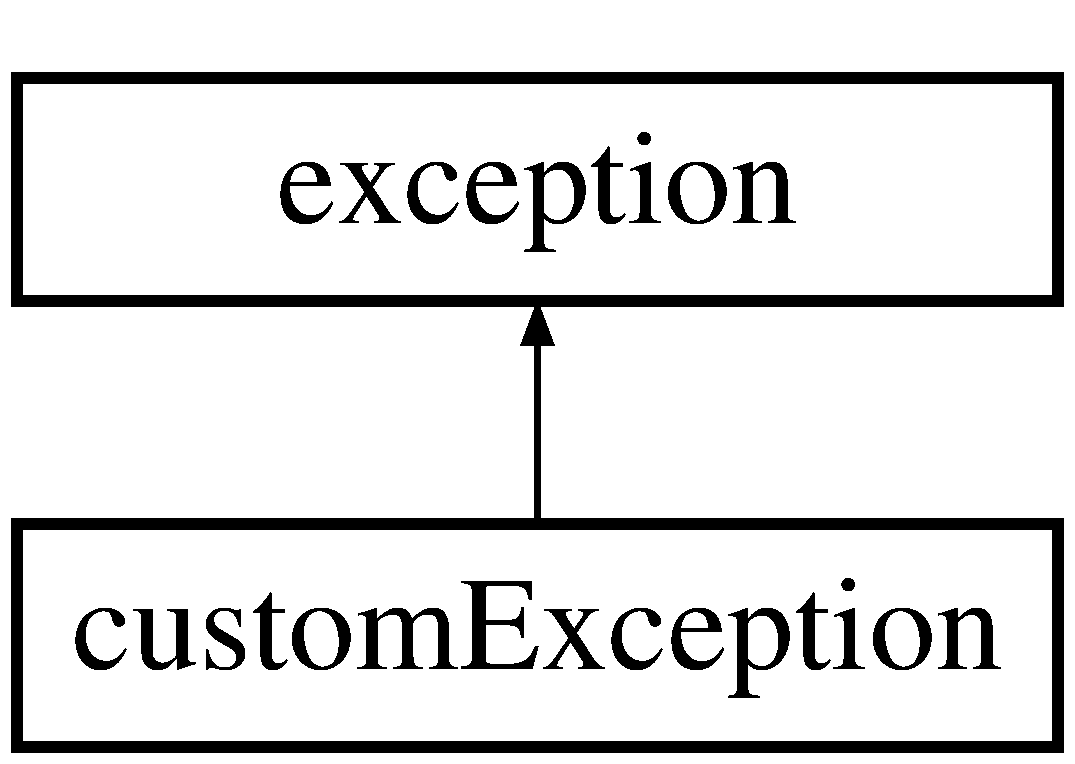
\includegraphics[height=2.000000cm]{classcustom_exception}
\end{center}
\end{figure}
\subsection*{Public Member Functions}
\begin{DoxyCompactItemize}
\item 
\hypertarget{classcustom_exception_aeb6ab5848b038adfc68fde86a512f691}{const char $\ast$ \hyperlink{classcustom_exception_aeb6ab5848b038adfc68fde86a512f691}{what} () const   throw ()}\label{classcustom_exception_aeb6ab5848b038adfc68fde86a512f691}

\begin{DoxyCompactList}\small\item\em Return a message pertaining to what went wrong. \end{DoxyCompactList}\item 
\hypertarget{classcustom_exception_a02ff9f09c4dd8c0b62fb1b6438d7d71a}{\hyperlink{classcustom_exception_a02ff9f09c4dd8c0b62fb1b6438d7d71a}{custom\-Exception} (std\-::string m=\char`\"{}custom exception occurred\char`\"{})}\label{classcustom_exception_a02ff9f09c4dd8c0b62fb1b6438d7d71a}

\begin{DoxyCompactList}\small\item\em Instantiate the object with a user specified message. \end{DoxyCompactList}\end{DoxyCompactItemize}


\subsection{Detailed Description}
Error reporting. 

Common values, structures, etc. \begin{DoxyAuthor}{Author}
Nathan A. Mahynski 
\end{DoxyAuthor}
\begin{DoxyDate}{Date}
11/17/13 
\end{DoxyDate}


Definition at line 14 of file common.\-h.



The documentation for this class was generated from the following file\-:\begin{DoxyCompactItemize}
\item 
/\-Users/nathanmahynski/\-C\-B\-E\-M\-D\-G\-P\-U/common.\-h\end{DoxyCompactItemize}

\hypertarget{structfloat3}{\section{float3 Struct Reference}
\label{structfloat3}\index{float3@{float3}}
}


3 floating point numbers, same as defined for G\-P\-Us  




{\ttfamily \#include $<$data\-Types.\-h$>$}

\subsection*{Public Attributes}
\begin{DoxyCompactItemize}
\item 
\hypertarget{structfloat3_af621f02abb1c788738fe61ea9807ff9c}{float {\bfseries x}}\label{structfloat3_af621f02abb1c788738fe61ea9807ff9c}

\item 
\hypertarget{structfloat3_aa6147d421a81889971f8c66aa92abf0d}{float {\bfseries y}}\label{structfloat3_aa6147d421a81889971f8c66aa92abf0d}

\item 
\hypertarget{structfloat3_a772dffd42d89f350c5a1b766c4703245}{float {\bfseries z}}\label{structfloat3_a772dffd42d89f350c5a1b766c4703245}

\end{DoxyCompactItemize}


\subsection{Detailed Description}
3 floating point numbers, same as defined for G\-P\-Us 

Requisite 'optimal' data types. \begin{DoxyDate}{Date}
11/21/13 
\end{DoxyDate}


Definition at line 15 of file data\-Types.\-h.



The documentation for this struct was generated from the following file\-:\begin{DoxyCompactItemize}
\item 
/\-Users/nathanmahynski/\-Desktop/\-C\-B\-E\-M\-D\-G\-P\-U/data\-Types.\-h\end{DoxyCompactItemize}

\hypertarget{structint3}{\section{int3 Struct Reference}
\label{structint3}\index{int3@{int3}}
}


3 integers, same as defined for G\-P\-Us  




{\ttfamily \#include $<$data\-Types.\-h$>$}

\subsection*{Public Attributes}
\begin{DoxyCompactItemize}
\item 
\hypertarget{structint3_a0a4ad50a155a35fa938ce6f16930affa}{int {\bfseries x}}\label{structint3_a0a4ad50a155a35fa938ce6f16930affa}

\item 
\hypertarget{structint3_a5d95e23491677d61019f0354b16adca9}{int {\bfseries y}}\label{structint3_a5d95e23491677d61019f0354b16adca9}

\item 
\hypertarget{structint3_a5cd5a3c388fa28814e3496ef07c39360}{int {\bfseries z}}\label{structint3_a5cd5a3c388fa28814e3496ef07c39360}

\end{DoxyCompactItemize}


\subsection{Detailed Description}
3 integers, same as defined for G\-P\-Us 

Definition at line 22 of file data\-Types.\-h.



The documentation for this struct was generated from the following file\-:\begin{DoxyCompactItemize}
\item 
/\-Users/nathanmahynski/\-C\-B\-E\-M\-D\-G\-P\-U/data\-Types.\-h\end{DoxyCompactItemize}

\hypertarget{classintegrator}{\section{integrator Class Reference}
\label{classintegrator}\index{integrator@{integrator}}
}


Base class for integrators such as N\-V\-T (Nose-\/\-Hoover) or N\-V\-E ensembles.  




{\ttfamily \#include $<$integrator.\-h$>$}

Inheritance diagram for integrator\-:\begin{figure}[H]
\begin{center}
\leavevmode
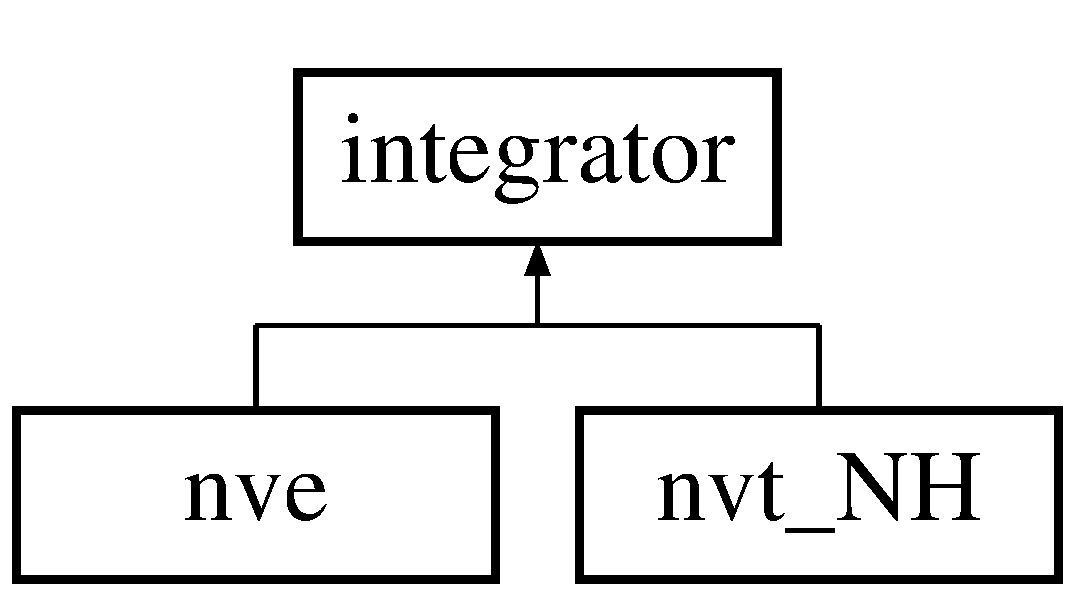
\includegraphics[height=2.000000cm]{classintegrator}
\end{center}
\end{figure}
\subsection*{Public Member Functions}
\begin{DoxyCompactItemize}
\item 
\hypertarget{classintegrator_a493bed6cf5d45fe41a9a6430bd063106}{void \hyperlink{classintegrator_a493bed6cf5d45fe41a9a6430bd063106}{set\-Timestep} (const float dt)}\label{classintegrator_a493bed6cf5d45fe41a9a6430bd063106}

\begin{DoxyCompactList}\small\item\em Set the integrator timestep. \end{DoxyCompactList}\item 
void \hyperlink{classintegrator_ad630bf7c9b7339fa34f36fe43b0d9e3c}{calc\-Force} (\hyperlink{classsystem_definition}{system\-Definition} \&sys)
\begin{DoxyCompactList}\small\item\em Calculate the forces on each atom. \end{DoxyCompactList}\item 
\hypertarget{classintegrator_a6f7170652474f15c99b94a9b9c7f4df6}{virtual void \hyperlink{classintegrator_a6f7170652474f15c99b94a9b9c7f4df6}{step} (\hyperlink{classsystem_definition}{system\-Definition} \&sys)=0}\label{classintegrator_a6f7170652474f15c99b94a9b9c7f4df6}

\begin{DoxyCompactList}\small\item\em Move the system forward a step in time. \end{DoxyCompactList}\end{DoxyCompactItemize}
\subsection*{Protected Attributes}
\begin{DoxyCompactItemize}
\item 
\hypertarget{classintegrator_ad1f7813c9cf3c31898aa7d78fc22232a}{\hyperlink{classcell_list__cpu}{cell\-List\-\_\-cpu} \hyperlink{classintegrator_ad1f7813c9cf3c31898aa7d78fc22232a}{cl\-\_\-}}\label{classintegrator_ad1f7813c9cf3c31898aa7d78fc22232a}

\begin{DoxyCompactList}\small\item\em Cell or neighbor list. \end{DoxyCompactList}\item 
\hypertarget{classintegrator_a3e183a65eb6a777479dca47e7f9a2676}{std\-::vector$<$ \hyperlink{structfloat3}{float3} $>$ \hyperlink{classintegrator_a3e183a65eb6a777479dca47e7f9a2676}{last\-Accelerations\-\_\-}}\label{classintegrator_a3e183a65eb6a777479dca47e7f9a2676}

\begin{DoxyCompactList}\small\item\em Acceleration of particles on previous timestep (useful for N\-V\-E integrator) \end{DoxyCompactList}\item 
\hypertarget{classintegrator_a6e4712b8597e3c40124316d2e9dd5051}{float \hyperlink{classintegrator_a6e4712b8597e3c40124316d2e9dd5051}{dt\-\_\-}}\label{classintegrator_a6e4712b8597e3c40124316d2e9dd5051}

\begin{DoxyCompactList}\small\item\em Timestep size. \end{DoxyCompactList}\item 
\hypertarget{classintegrator_a5b3546a765d8a83b6db8a6d890ace480}{int \hyperlink{classintegrator_a5b3546a765d8a83b6db8a6d890ace480}{start\-\_\-}}\label{classintegrator_a5b3546a765d8a83b6db8a6d890ace480}

\begin{DoxyCompactList}\small\item\em Flag for whether this object has been initialized or not. \end{DoxyCompactList}\end{DoxyCompactItemize}


\subsection{Detailed Description}
Base class for integrators such as N\-V\-T (Nose-\/\-Hoover) or N\-V\-E ensembles. 

Integrator \begin{DoxyAuthor}{Author}
Nathan A. Mahynski 
\end{DoxyAuthor}
\begin{DoxyDate}{Date}
11/17/13 
\end{DoxyDate}


Definition at line 15 of file integrator.\-h.



\subsection{Member Function Documentation}
\hypertarget{classintegrator_ad630bf7c9b7339fa34f36fe43b0d9e3c}{\index{integrator@{integrator}!calc\-Force@{calc\-Force}}
\index{calc\-Force@{calc\-Force}!integrator@{integrator}}
\subsubsection[{calc\-Force}]{\setlength{\rightskip}{0pt plus 5cm}void integrator\-::calc\-Force (
\begin{DoxyParamCaption}
\item[{{\bf system\-Definition} \&}]{sys}
\end{DoxyParamCaption}
)}}\label{classintegrator_ad630bf7c9b7339fa34f36fe43b0d9e3c}


Calculate the forces on each atom. 

Integration \begin{DoxyAuthor}{Author}
Nathan A. Mahynski 
\end{DoxyAuthor}
\begin{DoxyDate}{Date}
11/19/13
\end{DoxyDate}
Calculate the pairwise forces in a system. This also calculates the potential energy of a system. The kinetic energy is calculated during the verlet integration.


\begin{DoxyParams}[1]{Parameters}
\mbox{\tt in,out}  & {\em sys} & System definition\\
\hline
\end{DoxyParams}
Calculate the pairwise forces in a system. This also calculates the potential energy of a system. The kinetic energy is calculated during the verlet integration.


\begin{DoxyParams}[1]{Parameters}
\mbox{\tt in,out}  & {\em sys} & System definition \\
\hline
\end{DoxyParams}


Definition at line 23 of file integrator.\-cpp.



References system\-Definition\-::atoms, system\-Definition\-::box(), cell\-List\-\_\-cpu\-::check\-Update(), cl\-\_\-, cell\-List\-\_\-cpu\-::head(), cell\-List\-\_\-cpu\-::list(), system\-Definition\-::mass(), cell\-List\-\_\-cpu\-::n\-Cells, cell\-List\-\_\-cpu\-::neighbors(), system\-Definition\-::num\-Atoms(), system\-Definition\-::potential, system\-Definition\-::potential\-Args(), system\-Definition\-::rcut(), and system\-Definition\-::set\-Pot\-E().



Referenced by nve\-::step(), and nvt\-\_\-\-N\-H\-::step().


\begin{DoxyCode}
                                                 \{
    \textcolor{comment}{// For cache coeherency allocate new space for calculations}
    \hyperlink{structfloat3}{float3} empty;
    empty.x = 0; empty.y = 0; empty.z = 0;
    std::vector <float3> acc (sys.\hyperlink{classsystem_definition_ae8d3c2df2d56241cee03fcc4e2026ae0}{numAtoms}(), empty);
    \textcolor{keyword}{const} \textcolor{keywordtype}{float} rc = sys.\hyperlink{classsystem_definition_acacd88aac7d451bdcf9779ae8c5a95c7}{rcut}();

    \textcolor{comment}{// every time, check if the cell list needs to be updated first}
    \hyperlink{classintegrator_ad1f7813c9cf3c31898aa7d78fc22232a}{cl\_}.\hyperlink{classcell_list__cpu_a70568e6a2012eb8592f2798b3260c550}{checkUpdate}(sys);

    \textcolor{keywordtype}{float} Up = 0.0;
    \textcolor{keyword}{const} \hyperlink{structfloat3}{float3} box = sys.\hyperlink{classsystem_definition_a85b80dee3609ddb68e370cee3fa959ea}{box}();
    \textcolor{keyword}{const} \textcolor{keywordtype}{float} invMass = 1.0/sys.\hyperlink{classsystem_definition_acb6dd3df121e3e5bc0eb41c32bd937bd}{mass}();
    
    \textcolor{comment}{// traverse cell list and calculate total system potential energy }
    std::vector <float> args = sys.\hyperlink{classsystem_definition_ab20c0c30e84fccdf15f54c155d25420f}{potentialArgs}();
\textcolor{preprocessor}{#pragma omp parallel for reduction(+:Up) schedule(dynamic, 1)}
\textcolor{preprocessor}{}    \textcolor{keywordflow}{for} (\textcolor{keywordtype}{unsigned} \textcolor{keywordtype}{int} cellID = 0; cellID < \hyperlink{classintegrator_ad1f7813c9cf3c31898aa7d78fc22232a}{cl\_}.\hyperlink{classcell_list__cpu_ae86e1c9604a39bc8a493fa0f6538fd37}{nCells}.x*\hyperlink{classintegrator_ad1f7813c9cf3c31898aa7d78fc22232a}{cl\_}.\hyperlink{classcell_list__cpu_ae86e1c9604a39bc8a493fa0f6538fd37}{nCells}
      .y*\hyperlink{classintegrator_ad1f7813c9cf3c31898aa7d78fc22232a}{cl\_}.\hyperlink{classcell_list__cpu_ae86e1c9604a39bc8a493fa0f6538fd37}{nCells}.z; ++cellID) \{
        \textcolor{keywordtype}{int} atom1 = \hyperlink{classintegrator_ad1f7813c9cf3c31898aa7d78fc22232a}{cl\_}.\hyperlink{classcell_list__cpu_a0769d2a8a9c6964a8c6894bab9841e71}{head}(cellID);
        \textcolor{keywordflow}{while} (atom1 >= 0) \{
            std::vector < int > neighbors = \hyperlink{classintegrator_ad1f7813c9cf3c31898aa7d78fc22232a}{cl\_}.\hyperlink{classcell_list__cpu_aeaf165c887b13bfa7f7c1a8b70102aff}{neighbors}(cellID);
            \textcolor{keywordflow}{for} (\textcolor{keywordtype}{int} index = 0; index < neighbors.size(); ++index) \{
                \textcolor{keyword}{const} \textcolor{keywordtype}{int} cellID2 = neighbors[index];
                \textcolor{keywordtype}{int} atom2 = \hyperlink{classintegrator_ad1f7813c9cf3c31898aa7d78fc22232a}{cl\_}.\hyperlink{classcell_list__cpu_a0769d2a8a9c6964a8c6894bab9841e71}{head}(cellID2);
                \textcolor{keywordflow}{while} (atom2 >= 0) \{
                    \textcolor{keywordflow}{if} (atom1 > atom2) \{
                        \hyperlink{structfloat3}{float3} pf;
                        Up += sys.\hyperlink{classsystem_definition_a4861989c8ca1ddef7ec521499453df3f}{potential} (&sys.\hyperlink{classsystem_definition_ae8814d3f60fc1111af2a3f218a4bfcab}{atoms}[atom1].
      pos, &sys.\hyperlink{classsystem_definition_ae8814d3f60fc1111af2a3f218a4bfcab}{atoms}[atom2].pos, &pf, &box, &args[0], &rc);
                        acc[atom1].x -= pf.x*invMass; 
                        acc[atom1].y -= pf.y*invMass;
                        acc[atom1].z -= pf.z*invMass;
                        acc[atom2].x += pf.x*invMass;
                        acc[atom2].y += pf.y*invMass;
                        acc[atom2].z += pf.z*invMass;
                    \}
                    atom2 = \hyperlink{classintegrator_ad1f7813c9cf3c31898aa7d78fc22232a}{cl\_}.\hyperlink{classcell_list__cpu_ac274503e6cc75811e9cb9c07120fb96e}{list}(atom2);
                \}
            \}
            atom1 = \hyperlink{classintegrator_ad1f7813c9cf3c31898aa7d78fc22232a}{cl\_}.\hyperlink{classcell_list__cpu_ac274503e6cc75811e9cb9c07120fb96e}{list}(atom1);
        \}
    \}
    
    \textcolor{comment}{// save acceleration in array of atoms in system}
\textcolor{preprocessor}{    #pragma omp parallel for}
\textcolor{preprocessor}{}    \textcolor{keywordflow}{for} (\textcolor{keywordtype}{int} i = 0; i < sys.\hyperlink{classsystem_definition_ae8d3c2df2d56241cee03fcc4e2026ae0}{numAtoms}(); ++i) \{
        sys.\hyperlink{classsystem_definition_ae8814d3f60fc1111af2a3f218a4bfcab}{atoms}[i].acc.x = -acc[i].x;
        sys.\hyperlink{classsystem_definition_ae8814d3f60fc1111af2a3f218a4bfcab}{atoms}[i].acc.y = -acc[i].y;
        sys.\hyperlink{classsystem_definition_ae8814d3f60fc1111af2a3f218a4bfcab}{atoms}[i].acc.z = -acc[i].z;
    \}
    
    \textcolor{comment}{// set Up}
    sys.\hyperlink{classsystem_definition_a92a7d6457bd3f7ce71088e4df8e9ff4b}{setPotE}(Up);
\}
\end{DoxyCode}


The documentation for this class was generated from the following files\-:\begin{DoxyCompactItemize}
\item 
/\-Users/nathanmahynski/\-C\-B\-E\-M\-D\-G\-P\-U/integrator.\-h\item 
/\-Users/nathanmahynski/\-C\-B\-E\-M\-D\-G\-P\-U/integrator.\-cpp\item 
/\-Users/nathanmahynski/\-C\-B\-E\-M\-D\-G\-P\-U/integrator.\-cu\end{DoxyCompactItemize}

\hypertarget{classnve}{\section{nve Class Reference}
\label{classnve}\index{nve@{nve}}
}


Integration scheme that preserves total energy of the system.  




{\ttfamily \#include $<$nve.\-h$>$}

Inheritance diagram for nve\-:\begin{figure}[H]
\begin{center}
\leavevmode
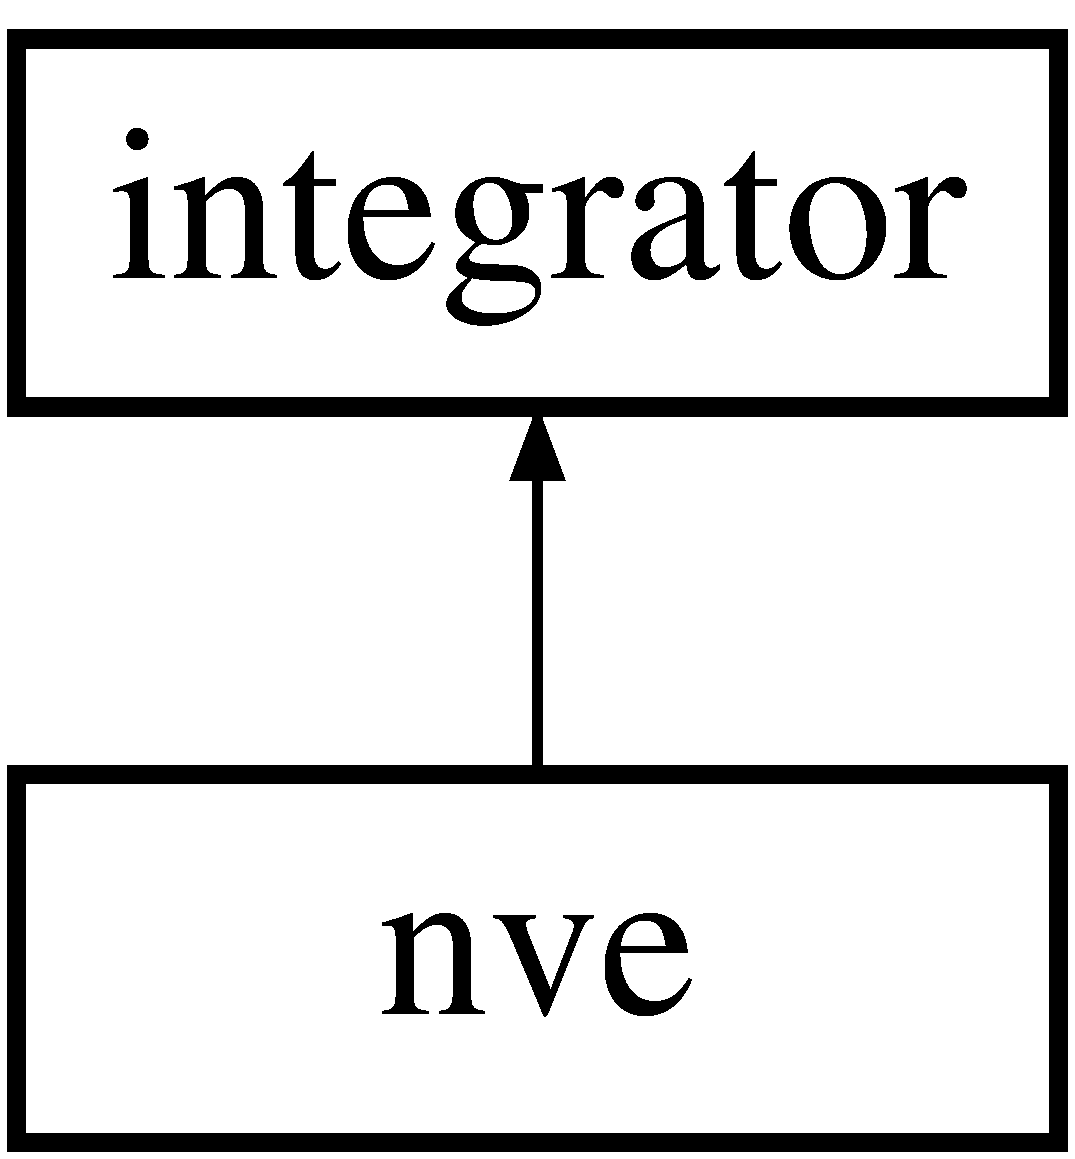
\includegraphics[height=2.000000cm]{classnve}
\end{center}
\end{figure}
\subsection*{Public Member Functions}
\begin{DoxyCompactItemize}
\item 
void \hyperlink{classnve_a4dddd7c0b5978d3d98e6a34e268558e0}{step} (\hyperlink{classsystem_definition}{system\-Definition} \&sys)
\item 
\hypertarget{classintegrator_a493bed6cf5d45fe41a9a6430bd063106}{void \hyperlink{classintegrator_a493bed6cf5d45fe41a9a6430bd063106}{set\-Timestep} (const float dt)}\label{classintegrator_a493bed6cf5d45fe41a9a6430bd063106}

\begin{DoxyCompactList}\small\item\em Set the integrator timestep. \end{DoxyCompactList}\item 
void \hyperlink{classintegrator_ad630bf7c9b7339fa34f36fe43b0d9e3c}{calc\-Force} (\hyperlink{classsystem_definition}{system\-Definition} \&sys)
\begin{DoxyCompactList}\small\item\em Calculate the forces on each atom. \end{DoxyCompactList}\end{DoxyCompactItemize}
\subsection*{Protected Attributes}
\begin{DoxyCompactItemize}
\item 
\hypertarget{classintegrator_ad1f7813c9cf3c31898aa7d78fc22232a}{\hyperlink{classcell_list__cpu}{cell\-List\-\_\-cpu} \hyperlink{classintegrator_ad1f7813c9cf3c31898aa7d78fc22232a}{cl\-\_\-}}\label{classintegrator_ad1f7813c9cf3c31898aa7d78fc22232a}

\begin{DoxyCompactList}\small\item\em Cell or neighbor list. \end{DoxyCompactList}\item 
\hypertarget{classintegrator_a3e183a65eb6a777479dca47e7f9a2676}{std\-::vector$<$ \hyperlink{structfloat3}{float3} $>$ \hyperlink{classintegrator_a3e183a65eb6a777479dca47e7f9a2676}{last\-Accelerations\-\_\-}}\label{classintegrator_a3e183a65eb6a777479dca47e7f9a2676}

\begin{DoxyCompactList}\small\item\em Acceleration of particles on previous timestep (useful for N\-V\-E integrator) \end{DoxyCompactList}\item 
\hypertarget{classintegrator_a6e4712b8597e3c40124316d2e9dd5051}{float \hyperlink{classintegrator_a6e4712b8597e3c40124316d2e9dd5051}{dt\-\_\-}}\label{classintegrator_a6e4712b8597e3c40124316d2e9dd5051}

\begin{DoxyCompactList}\small\item\em Timestep size. \end{DoxyCompactList}\item 
\hypertarget{classintegrator_a5b3546a765d8a83b6db8a6d890ace480}{int \hyperlink{classintegrator_a5b3546a765d8a83b6db8a6d890ace480}{start\-\_\-}}\label{classintegrator_a5b3546a765d8a83b6db8a6d890ace480}

\begin{DoxyCompactList}\small\item\em Flag for whether this object has been initialized or not. \end{DoxyCompactList}\end{DoxyCompactItemize}


\subsection{Detailed Description}
Integration scheme that preserves total energy of the system. 

N\-V\-E integration. \begin{DoxyDate}{Date}
11/18/13 
\end{DoxyDate}


Definition at line 13 of file nve.\-h.



\subsection{Member Function Documentation}
\hypertarget{classintegrator_ad630bf7c9b7339fa34f36fe43b0d9e3c}{\index{nve@{nve}!calc\-Force@{calc\-Force}}
\index{calc\-Force@{calc\-Force}!nve@{nve}}
\subsubsection[{calc\-Force}]{\setlength{\rightskip}{0pt plus 5cm}void integrator\-::calc\-Force (
\begin{DoxyParamCaption}
\item[{{\bf system\-Definition} \&}]{sys}
\end{DoxyParamCaption}
)\hspace{0.3cm}{\ttfamily [inherited]}}}\label{classintegrator_ad630bf7c9b7339fa34f36fe43b0d9e3c}


Calculate the forces on each atom. 

Integration \begin{DoxyDate}{Date}
11/19/13
\end{DoxyDate}
Calculate the pairwise forces in a system. This also calculates the potential energy of a system. The kinetic energy is calculated during the verlet integration.


\begin{DoxyParams}[1]{Parameters}
\mbox{\tt in,out}  & {\em sys} & System definition \\
\hline
\end{DoxyParams}


Definition at line 22 of file integrator.\-cpp.



References system\-Definition\-::atoms, system\-Definition\-::box(), cell\-List\-\_\-cpu\-::check\-Update(), integrator\-::cl\-\_\-, cell\-List\-\_\-cpu\-::head(), cell\-List\-\_\-cpu\-::list(), system\-Definition\-::mass(), cell\-List\-\_\-cpu\-::n\-Cells, cell\-List\-\_\-cpu\-::neighbors(), system\-Definition\-::num\-Atoms(), system\-Definition\-::potential, system\-Definition\-::potential\-Args(), system\-Definition\-::rcut(), and system\-Definition\-::set\-Pot\-E().



Referenced by step(), and nvt\-\_\-\-N\-H\-::step().


\begin{DoxyCode}
                                                 \{
    \textcolor{comment}{// For cache coeherency allocate new space for calculations}
    \hyperlink{structfloat3}{float3} empty;
    empty.x = 0; empty.y = 0; empty.z = 0;
    std::vector <float3> acc (sys.\hyperlink{classsystem_definition_ae8d3c2df2d56241cee03fcc4e2026ae0}{numAtoms}(), empty);
    \textcolor{keyword}{const} \textcolor{keywordtype}{float} rc = sys.\hyperlink{classsystem_definition_acacd88aac7d451bdcf9779ae8c5a95c7}{rcut}();

    \textcolor{comment}{// every time, check if the cell list needs to be updated first}
    \hyperlink{classintegrator_ad1f7813c9cf3c31898aa7d78fc22232a}{cl\_}.\hyperlink{classcell_list__cpu_a70568e6a2012eb8592f2798b3260c550}{checkUpdate}(sys);

    \textcolor{keywordtype}{float} Up = 0.0;
    \textcolor{keyword}{const} \hyperlink{structfloat3}{float3} box = sys.\hyperlink{classsystem_definition_a85b80dee3609ddb68e370cee3fa959ea}{box}();
    \textcolor{keyword}{const} \textcolor{keywordtype}{float} invMass = 1.0/sys.\hyperlink{classsystem_definition_acb6dd3df121e3e5bc0eb41c32bd937bd}{mass}();
    
    \textcolor{comment}{// traverse cell list and calculate total system potential energy }
    std::vector <float> args = sys.\hyperlink{classsystem_definition_ab20c0c30e84fccdf15f54c155d25420f}{potentialArgs}();
\textcolor{preprocessor}{    #pragma omp parallel for reduction(+:Up) schedule(dynamic, 1)}
\textcolor{preprocessor}{}    \textcolor{keywordflow}{for} (\textcolor{keywordtype}{unsigned} \textcolor{keywordtype}{int} cellID = 0; cellID < \hyperlink{classintegrator_ad1f7813c9cf3c31898aa7d78fc22232a}{cl\_}.\hyperlink{classcell_list__cpu_ae86e1c9604a39bc8a493fa0f6538fd37}{nCells}.x*\hyperlink{classintegrator_ad1f7813c9cf3c31898aa7d78fc22232a}{cl\_}.\hyperlink{classcell_list__cpu_ae86e1c9604a39bc8a493fa0f6538fd37}{nCells}
      .y*\hyperlink{classintegrator_ad1f7813c9cf3c31898aa7d78fc22232a}{cl\_}.\hyperlink{classcell_list__cpu_ae86e1c9604a39bc8a493fa0f6538fd37}{nCells}.z; ++cellID) \{
        \textcolor{keywordtype}{int} atom1 = \hyperlink{classintegrator_ad1f7813c9cf3c31898aa7d78fc22232a}{cl\_}.\hyperlink{classcell_list__cpu_a0769d2a8a9c6964a8c6894bab9841e71}{head}(cellID);
        \textcolor{keywordflow}{while} (atom1 >= 0) \{
            std::vector < int > neighbors = \hyperlink{classintegrator_ad1f7813c9cf3c31898aa7d78fc22232a}{cl\_}.\hyperlink{classcell_list__cpu_aeaf165c887b13bfa7f7c1a8b70102aff}{neighbors}(cellID);
            \textcolor{keywordflow}{for} (\textcolor{keywordtype}{int} index = 0; index < neighbors.size(); ++index) \{
                \textcolor{keyword}{const} \textcolor{keywordtype}{int} cellID2 = neighbors[index];
                \textcolor{keywordtype}{int} atom2 = \hyperlink{classintegrator_ad1f7813c9cf3c31898aa7d78fc22232a}{cl\_}.\hyperlink{classcell_list__cpu_a0769d2a8a9c6964a8c6894bab9841e71}{head}(cellID2);
                \textcolor{keywordflow}{while} (atom2 >= 0) \{
                    \textcolor{keywordflow}{if} (atom1 > atom2) \{
                        \hyperlink{structfloat3}{float3} pf;
                        Up += sys.\hyperlink{classsystem_definition_a4861989c8ca1ddef7ec521499453df3f}{potential} (&sys.\hyperlink{classsystem_definition_ae8814d3f60fc1111af2a3f218a4bfcab}{atoms}[atom1].
      pos, &sys.\hyperlink{classsystem_definition_ae8814d3f60fc1111af2a3f218a4bfcab}{atoms}[atom2].pos, &pf, &box, &args[0], &rc);
                        acc[atom1].x -= pf.x*invMass; 
                        acc[atom1].y -= pf.y*invMass;
                        acc[atom1].z -= pf.z*invMass;
                        acc[atom2].x += pf.x*invMass;
                        acc[atom2].y += pf.y*invMass;
                        acc[atom2].z += pf.z*invMass;
                    \}
                    atom2 = \hyperlink{classintegrator_ad1f7813c9cf3c31898aa7d78fc22232a}{cl\_}.\hyperlink{classcell_list__cpu_ac274503e6cc75811e9cb9c07120fb96e}{list}(atom2);
                \}
            \}
            atom1 = \hyperlink{classintegrator_ad1f7813c9cf3c31898aa7d78fc22232a}{cl\_}.\hyperlink{classcell_list__cpu_ac274503e6cc75811e9cb9c07120fb96e}{list}(atom1);
        \}
    \}
    
    \textcolor{comment}{// save acceleration in array of atoms in system}
\textcolor{preprocessor}{    #pragma omp parallel for}
\textcolor{preprocessor}{}    \textcolor{keywordflow}{for} (\textcolor{keywordtype}{int} i = 0; i < sys.\hyperlink{classsystem_definition_ae8d3c2df2d56241cee03fcc4e2026ae0}{numAtoms}(); ++i) \{
        sys.\hyperlink{classsystem_definition_ae8814d3f60fc1111af2a3f218a4bfcab}{atoms}[i].acc.x = -acc[i].x;
        sys.\hyperlink{classsystem_definition_ae8814d3f60fc1111af2a3f218a4bfcab}{atoms}[i].acc.y = -acc[i].y;
        sys.\hyperlink{classsystem_definition_ae8814d3f60fc1111af2a3f218a4bfcab}{atoms}[i].acc.z = -acc[i].z;
    \}
    
    \textcolor{comment}{// set Up}
    sys.\hyperlink{classsystem_definition_a92a7d6457bd3f7ce71088e4df8e9ff4b}{setPotE}(Up);
\}
\end{DoxyCode}
\hypertarget{classnve_a4dddd7c0b5978d3d98e6a34e268558e0}{\index{nve@{nve}!step@{step}}
\index{step@{step}!nve@{nve}}
\subsubsection[{step}]{\setlength{\rightskip}{0pt plus 5cm}void nve\-::step (
\begin{DoxyParamCaption}
\item[{{\bf system\-Definition} \&}]{sys}
\end{DoxyParamCaption}
)\hspace{0.3cm}{\ttfamily [virtual]}}}\label{classnve_a4dddd7c0b5978d3d98e6a34e268558e0}
Do N\-V\-E integration \begin{DoxyDate}{Date}
11/18/13
\end{DoxyDate}
Integrate a single timestep forward using Velocity-\/\-Verlet integration scheme. Update the positions and velocities using velocity verlet integration. This uses the accelerations stored on each atom. Creates a cell list the first time it is called. 
\begin{DoxyParams}[1]{Parameters}
\mbox{\tt in,out}  & {\em sys} & System definition \\
\hline
\end{DoxyParams}


Implements \hyperlink{classintegrator_a6f7170652474f15c99b94a9b9c7f4df6}{integrator}.



Definition at line 22 of file nve.\-cpp.



References system\-Definition\-::atoms, integrator\-::calc\-Force(), integrator\-::dt\-\_\-, integrator\-::last\-Accelerations\-\_\-, system\-Definition\-::mass(), system\-Definition\-::num\-Atoms(), system\-Definition\-::set\-Kin\-E(), integrator\-::start\-\_\-, and system\-Definition\-::update\-Instant\-Temp().


\begin{DoxyCode}
                                     \{
    \textcolor{keywordflow}{if} (\hyperlink{classintegrator_a5b3546a765d8a83b6db8a6d890ace480}{start\_}) \{
        \textcolor{keywordflow}{try} \{
            \hyperlink{classintegrator_a3e183a65eb6a777479dca47e7f9a2676}{lastAccelerations\_}.resize(sys.\hyperlink{classsystem_definition_ae8d3c2df2d56241cee03fcc4e2026ae0}{numAtoms}())
      ;
        \} \textcolor{keywordflow}{catch} (std::exception &e) \{
            std::cerr << e.what() << std::endl;
            \textcolor{keywordflow}{throw} \hyperlink{classcustom_exception}{customException}(\textcolor{stringliteral}{"Failed to initialize
       integrator due to memory constraints"});
            \textcolor{keywordflow}{return};
        \}
        \textcolor{comment}{// calculate the forces initially (sets Up)}
        \hyperlink{classintegrator_ad630bf7c9b7339fa34f36fe43b0d9e3c}{calcForce} (sys);
        
        \textcolor{comment}{// also get initial T}
\textcolor{preprocessor}{        #pragma omp parallel}
\textcolor{preprocessor}{}        \{
\textcolor{preprocessor}{            #pragma omp for shared(sys.atoms) schedule(dynamic, OMP\_CHUNK) }
\textcolor{preprocessor}{}            \textcolor{keywordflow}{for} (\textcolor{keywordtype}{unsigned} \textcolor{keywordtype}{int} i = 0; i < sys.\hyperlink{classsystem_definition_ae8d3c2df2d56241cee03fcc4e2026ae0}{numAtoms}(); ++i) \{
                sys.\hyperlink{classsystem_definition_ae8814d3f60fc1111af2a3f218a4bfcab}{atoms}[i].vel.x += \hyperlink{classintegrator_a6e4712b8597e3c40124316d2e9dd5051}{dt\_}*0.5*(\hyperlink{classintegrator_a3e183a65eb6a777479dca47e7f9a2676}{lastAccelerations\_}
      [i].x+sys.\hyperlink{classsystem_definition_ae8814d3f60fc1111af2a3f218a4bfcab}{atoms}[i].acc.x);
                sys.\hyperlink{classsystem_definition_ae8814d3f60fc1111af2a3f218a4bfcab}{atoms}[i].vel.y += \hyperlink{classintegrator_a6e4712b8597e3c40124316d2e9dd5051}{dt\_}*0.5*(\hyperlink{classintegrator_a3e183a65eb6a777479dca47e7f9a2676}{lastAccelerations\_}
      [i].y+sys.\hyperlink{classsystem_definition_ae8814d3f60fc1111af2a3f218a4bfcab}{atoms}[i].acc.y);
                sys.\hyperlink{classsystem_definition_ae8814d3f60fc1111af2a3f218a4bfcab}{atoms}[i].vel.z += \hyperlink{classintegrator_a6e4712b8597e3c40124316d2e9dd5051}{dt\_}*0.5*(\hyperlink{classintegrator_a3e183a65eb6a777479dca47e7f9a2676}{lastAccelerations\_}
      [i].z+sys.\hyperlink{classsystem_definition_ae8814d3f60fc1111af2a3f218a4bfcab}{atoms}[i].acc.z);
            \}
        \}
        
        \textcolor{keywordtype}{float} tmp = 0.0, Uk = 0.0;
\textcolor{preprocessor}{        #pragma omp parallel}
\textcolor{preprocessor}{}        \{
\textcolor{preprocessor}{            #pragma omp reduction(+:Uk) schedule(dynamic, OMP\_CHUNK) }
\textcolor{preprocessor}{}            \textcolor{keywordflow}{for} (\textcolor{keywordtype}{unsigned} \textcolor{keywordtype}{int} i = 0; i < sys.\hyperlink{classsystem_definition_ae8d3c2df2d56241cee03fcc4e2026ae0}{numAtoms}(); ++i) \{
                Uk += (sys.\hyperlink{classsystem_definition_ae8814d3f60fc1111af2a3f218a4bfcab}{atoms}[i].vel.x*sys.\hyperlink{classsystem_definition_ae8814d3f60fc1111af2a3f218a4bfcab}{atoms}[i].vel.x)+(sys.
      \hyperlink{classsystem_definition_ae8814d3f60fc1111af2a3f218a4bfcab}{atoms}[i].vel.y*sys.\hyperlink{classsystem_definition_ae8814d3f60fc1111af2a3f218a4bfcab}{atoms}[i].vel.y)+(sys.\hyperlink{classsystem_definition_ae8814d3f60fc1111af2a3f218a4bfcab}{atoms}[i].vel.z*sys.\hyperlink{classsystem_definition_ae8814d3f60fc1111af2a3f218a4bfcab}{atoms}
      [i].vel.z);
            \}
        \}
        Uk *= sys.\hyperlink{classsystem_definition_acb6dd3df121e3e5bc0eb41c32bd937bd}{mass}();
        tmp = Uk;
        Uk *= 0.5;
        tmp /= (3.0*(sys.\hyperlink{classsystem_definition_ae8d3c2df2d56241cee03fcc4e2026ae0}{numAtoms}()-1.0));
        sys.\hyperlink{classsystem_definition_a285e6cd1de35ed125eecb20f0f774ab3}{updateInstantTemp}(tmp);
        sys.\hyperlink{classsystem_definition_a2b2c236698886bd1d106be802b987b61}{setKinE}(Uk);
        \hyperlink{classintegrator_a5b3546a765d8a83b6db8a6d890ace480}{start\_} = 0;
    \}
    
    \textcolor{comment}{// update positions based on current positions}
\textcolor{preprocessor}{    #pragma omp parallel}
\textcolor{preprocessor}{}    \{
\textcolor{preprocessor}{        #pragma omp for shared(sys.atoms) schedule(dynamic, OMP\_CHUNK) }
\textcolor{preprocessor}{}        \textcolor{keywordflow}{for} (\textcolor{keywordtype}{unsigned} \textcolor{keywordtype}{int} i = 0; i < sys.\hyperlink{classsystem_definition_ae8d3c2df2d56241cee03fcc4e2026ae0}{numAtoms}(); ++i) \{
            sys.\hyperlink{classsystem_definition_ae8814d3f60fc1111af2a3f218a4bfcab}{atoms}[i].pos.x += \hyperlink{classintegrator_a6e4712b8597e3c40124316d2e9dd5051}{dt\_}*(sys.\hyperlink{classsystem_definition_ae8814d3f60fc1111af2a3f218a4bfcab}{atoms}[i].vel.x+0.5*\hyperlink{classintegrator_a6e4712b8597e3c40124316d2e9dd5051}{dt\_}
      *sys.\hyperlink{classsystem_definition_ae8814d3f60fc1111af2a3f218a4bfcab}{atoms}[i].acc.x);
            sys.\hyperlink{classsystem_definition_ae8814d3f60fc1111af2a3f218a4bfcab}{atoms}[i].pos.y += \hyperlink{classintegrator_a6e4712b8597e3c40124316d2e9dd5051}{dt\_}*(sys.\hyperlink{classsystem_definition_ae8814d3f60fc1111af2a3f218a4bfcab}{atoms}[i].vel.y+0.5*\hyperlink{classintegrator_a6e4712b8597e3c40124316d2e9dd5051}{dt\_}
      *sys.\hyperlink{classsystem_definition_ae8814d3f60fc1111af2a3f218a4bfcab}{atoms}[i].acc.y);
            sys.\hyperlink{classsystem_definition_ae8814d3f60fc1111af2a3f218a4bfcab}{atoms}[i].pos.z += \hyperlink{classintegrator_a6e4712b8597e3c40124316d2e9dd5051}{dt\_}*(sys.\hyperlink{classsystem_definition_ae8814d3f60fc1111af2a3f218a4bfcab}{atoms}[i].vel.z+0.5*\hyperlink{classintegrator_a6e4712b8597e3c40124316d2e9dd5051}{dt\_}
      *sys.\hyperlink{classsystem_definition_ae8814d3f60fc1111af2a3f218a4bfcab}{atoms}[i].acc.z);
            \hyperlink{classintegrator_a3e183a65eb6a777479dca47e7f9a2676}{lastAccelerations\_}[i] = sys.\hyperlink{classsystem_definition_ae8814d3f60fc1111af2a3f218a4bfcab}{atoms}[i].acc;
        \}
    \}
    
    \textcolor{comment}{// calculate new forces at new positions}
    \hyperlink{classintegrator_ad630bf7c9b7339fa34f36fe43b0d9e3c}{calcForce} (sys);
    
    \textcolor{comment}{// update velocities and get Uk and kinetic temperature}
\textcolor{preprocessor}{    #pragma omp parallel}
\textcolor{preprocessor}{}    \{
\textcolor{preprocessor}{        #pragma omp for shared(sys.atoms) schedule(dynamic, OMP\_CHUNK) }
\textcolor{preprocessor}{}        \textcolor{keywordflow}{for} (\textcolor{keywordtype}{unsigned} \textcolor{keywordtype}{int} i = 0; i < sys.\hyperlink{classsystem_definition_ae8d3c2df2d56241cee03fcc4e2026ae0}{numAtoms}(); ++i) \{
            sys.\hyperlink{classsystem_definition_ae8814d3f60fc1111af2a3f218a4bfcab}{atoms}[i].vel.x += \hyperlink{classintegrator_a6e4712b8597e3c40124316d2e9dd5051}{dt\_}*0.5*(\hyperlink{classintegrator_a3e183a65eb6a777479dca47e7f9a2676}{lastAccelerations\_}
      [i].x+sys.\hyperlink{classsystem_definition_ae8814d3f60fc1111af2a3f218a4bfcab}{atoms}[i].acc.x);
            sys.\hyperlink{classsystem_definition_ae8814d3f60fc1111af2a3f218a4bfcab}{atoms}[i].vel.y += \hyperlink{classintegrator_a6e4712b8597e3c40124316d2e9dd5051}{dt\_}*0.5*(\hyperlink{classintegrator_a3e183a65eb6a777479dca47e7f9a2676}{lastAccelerations\_}
      [i].y+sys.\hyperlink{classsystem_definition_ae8814d3f60fc1111af2a3f218a4bfcab}{atoms}[i].acc.y);
            sys.\hyperlink{classsystem_definition_ae8814d3f60fc1111af2a3f218a4bfcab}{atoms}[i].vel.z += \hyperlink{classintegrator_a6e4712b8597e3c40124316d2e9dd5051}{dt\_}*0.5*(\hyperlink{classintegrator_a3e183a65eb6a777479dca47e7f9a2676}{lastAccelerations\_}
      [i].z+sys.\hyperlink{classsystem_definition_ae8814d3f60fc1111af2a3f218a4bfcab}{atoms}[i].acc.z);
        \}
    \}
    
    \textcolor{comment}{// get temperature and kinetic energy}
    \textcolor{keywordtype}{float} tmp = 0.0, Uk = 0.0;
\textcolor{preprocessor}{    #pragma omp parallel}
\textcolor{preprocessor}{}    \{
\textcolor{preprocessor}{        #pragma omp reduction(+:Uk) schedule(dynamic, OMP\_CHUNK) }
\textcolor{preprocessor}{}        \textcolor{keywordflow}{for} (\textcolor{keywordtype}{unsigned} \textcolor{keywordtype}{int} i = 0; i < sys.\hyperlink{classsystem_definition_ae8d3c2df2d56241cee03fcc4e2026ae0}{numAtoms}(); ++i) \{
            Uk += (sys.\hyperlink{classsystem_definition_ae8814d3f60fc1111af2a3f218a4bfcab}{atoms}[i].vel.x*sys.\hyperlink{classsystem_definition_ae8814d3f60fc1111af2a3f218a4bfcab}{atoms}[i].vel.x)+(sys.\hyperlink{classsystem_definition_ae8814d3f60fc1111af2a3f218a4bfcab}{atoms}
      [i].vel.y*sys.\hyperlink{classsystem_definition_ae8814d3f60fc1111af2a3f218a4bfcab}{atoms}[i].vel.y)+(sys.\hyperlink{classsystem_definition_ae8814d3f60fc1111af2a3f218a4bfcab}{atoms}[i].vel.z*sys.\hyperlink{classsystem_definition_ae8814d3f60fc1111af2a3f218a4bfcab}{atoms}[i].
      vel.z);
        \}
    \}
    Uk *= sys.\hyperlink{classsystem_definition_acb6dd3df121e3e5bc0eb41c32bd937bd}{mass}();
    tmp = Uk;
    Uk *= 0.5;
    tmp /= (3.0*(sys.\hyperlink{classsystem_definition_ae8d3c2df2d56241cee03fcc4e2026ae0}{numAtoms}()-1.0));
    sys.\hyperlink{classsystem_definition_a285e6cd1de35ed125eecb20f0f774ab3}{updateInstantTemp}(tmp);
    sys.\hyperlink{classsystem_definition_a2b2c236698886bd1d106be802b987b61}{setKinE}(Uk);
\}
\end{DoxyCode}


The documentation for this class was generated from the following files\-:\begin{DoxyCompactItemize}
\item 
/\-Users/nathanmahynski/\-Desktop/\-C\-B\-E\-M\-D\-G\-P\-U/nve.\-h\item 
/\-Users/nathanmahynski/\-Desktop/\-C\-B\-E\-M\-D\-G\-P\-U/nve.\-cpp\end{DoxyCompactItemize}

\hypertarget{classnvt___n_h}{\section{nvt\-\_\-\-N\-H Class Reference}
\label{classnvt___n_h}\index{nvt\-\_\-\-N\-H@{nvt\-\_\-\-N\-H}}
}


Uses Nose-\/\-Hover integration method to thermostat a system (constant T rather than E)  




{\ttfamily \#include $<$nvt.\-h$>$}

Inheritance diagram for nvt\-\_\-\-N\-H\-:\begin{figure}[H]
\begin{center}
\leavevmode
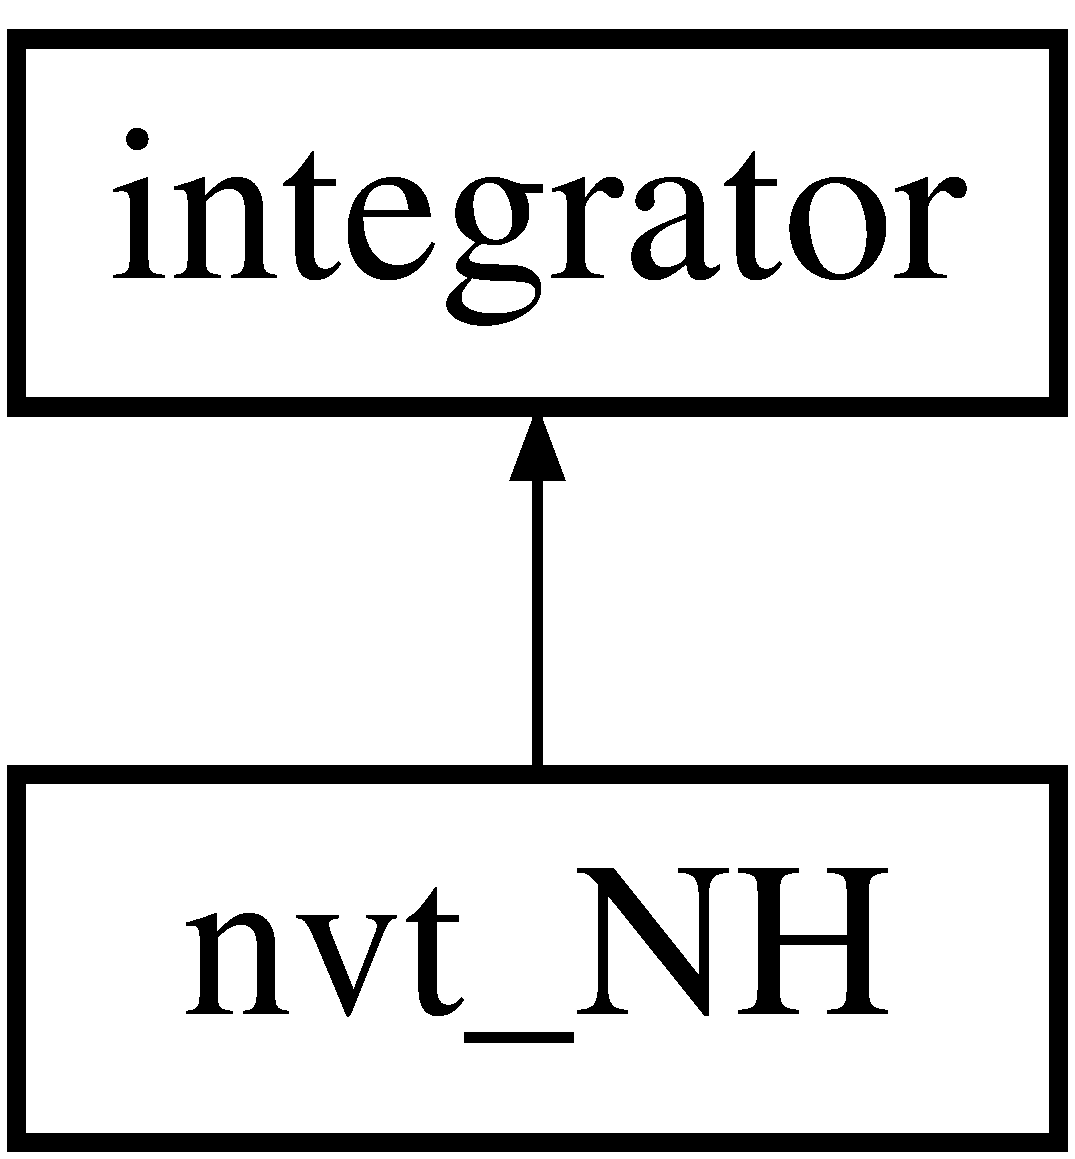
\includegraphics[height=2.000000cm]{classnvt___n_h}
\end{center}
\end{figure}
\subsection*{Public Member Functions}
\begin{DoxyCompactItemize}
\item 
\hyperlink{classnvt___n_h_a2de57e4e2a370bbfc8c0026963352ef1}{nvt\-\_\-\-N\-H} (const float Q)
\item 
void \hyperlink{classnvt___n_h_aa5b74d6b986c65e4436fed6ea6c14b20}{step} (\hyperlink{classsystem_definition}{system\-Definition} \&sys)
\item 
\hypertarget{classintegrator_a493bed6cf5d45fe41a9a6430bd063106}{void \hyperlink{classintegrator_a493bed6cf5d45fe41a9a6430bd063106}{set\-Timestep} (const float dt)}\label{classintegrator_a493bed6cf5d45fe41a9a6430bd063106}

\begin{DoxyCompactList}\small\item\em Set the integrator timestep. \end{DoxyCompactList}\item 
void \hyperlink{classintegrator_ad630bf7c9b7339fa34f36fe43b0d9e3c}{calc\-Force} (\hyperlink{classsystem_definition}{system\-Definition} \&sys)
\begin{DoxyCompactList}\small\item\em Calculate the forces on each atom. \end{DoxyCompactList}\end{DoxyCompactItemize}
\subsection*{Protected Attributes}
\begin{DoxyCompactItemize}
\item 
\hypertarget{classintegrator_ad1f7813c9cf3c31898aa7d78fc22232a}{\hyperlink{classcell_list__cpu}{cell\-List\-\_\-cpu} \hyperlink{classintegrator_ad1f7813c9cf3c31898aa7d78fc22232a}{cl\-\_\-}}\label{classintegrator_ad1f7813c9cf3c31898aa7d78fc22232a}

\begin{DoxyCompactList}\small\item\em Cell or neighbor list. \end{DoxyCompactList}\item 
\hypertarget{classintegrator_a3e183a65eb6a777479dca47e7f9a2676}{std\-::vector$<$ \hyperlink{structfloat3}{float3} $>$ \hyperlink{classintegrator_a3e183a65eb6a777479dca47e7f9a2676}{last\-Accelerations\-\_\-}}\label{classintegrator_a3e183a65eb6a777479dca47e7f9a2676}

\begin{DoxyCompactList}\small\item\em Acceleration of particles on previous timestep (useful for N\-V\-E integrator) \end{DoxyCompactList}\item 
\hypertarget{classintegrator_a6e4712b8597e3c40124316d2e9dd5051}{float \hyperlink{classintegrator_a6e4712b8597e3c40124316d2e9dd5051}{dt\-\_\-}}\label{classintegrator_a6e4712b8597e3c40124316d2e9dd5051}

\begin{DoxyCompactList}\small\item\em Timestep size. \end{DoxyCompactList}\item 
\hypertarget{classintegrator_a5b3546a765d8a83b6db8a6d890ace480}{int \hyperlink{classintegrator_a5b3546a765d8a83b6db8a6d890ace480}{start\-\_\-}}\label{classintegrator_a5b3546a765d8a83b6db8a6d890ace480}

\begin{DoxyCompactList}\small\item\em Flag for whether this object has been initialized or not. \end{DoxyCompactList}\end{DoxyCompactItemize}


\subsection{Detailed Description}
Uses Nose-\/\-Hover integration method to thermostat a system (constant T rather than E) 

N\-V\-T integration with Nose-\/\-Hoover thermostat. \begin{DoxyDate}{Date}
11/18/13 
\end{DoxyDate}


Definition at line 13 of file nvt.\-h.



\subsection{Constructor \& Destructor Documentation}
\hypertarget{classnvt___n_h_a2de57e4e2a370bbfc8c0026963352ef1}{\index{nvt\-\_\-\-N\-H@{nvt\-\_\-\-N\-H}!nvt\-\_\-\-N\-H@{nvt\-\_\-\-N\-H}}
\index{nvt\-\_\-\-N\-H@{nvt\-\_\-\-N\-H}!nvt_NH@{nvt\-\_\-\-N\-H}}
\subsubsection[{nvt\-\_\-\-N\-H}]{\setlength{\rightskip}{0pt plus 5cm}nvt\-\_\-\-N\-H\-::nvt\-\_\-\-N\-H (
\begin{DoxyParamCaption}
\item[{const float}]{Q}
\end{DoxyParamCaption}
)}}\label{classnvt___n_h_a2de57e4e2a370bbfc8c0026963352ef1}
Do N\-V\-T integration with Nose-\/\-Hoover thermostat. \begin{DoxyDate}{Date}
11/18/13
\end{DoxyDate}
Initialize integrator


\begin{DoxyParams}[1]{Parameters}
\mbox{\tt in}  & {\em Q} & Thermal mass for thermostat \\
\hline
\end{DoxyParams}


Definition at line 20 of file nvt.\-cpp.



References integrator\-::start\-\_\-.


\begin{DoxyCode}
                             \{
    Q\_ = Q; 
    gamma\_ = 0.0;
    \hyperlink{classintegrator_a5b3546a765d8a83b6db8a6d890ace480}{start\_} = 1; 
\}
\end{DoxyCode}


\subsection{Member Function Documentation}
\hypertarget{classintegrator_ad630bf7c9b7339fa34f36fe43b0d9e3c}{\index{nvt\-\_\-\-N\-H@{nvt\-\_\-\-N\-H}!calc\-Force@{calc\-Force}}
\index{calc\-Force@{calc\-Force}!nvt_NH@{nvt\-\_\-\-N\-H}}
\subsubsection[{calc\-Force}]{\setlength{\rightskip}{0pt plus 5cm}void integrator\-::calc\-Force (
\begin{DoxyParamCaption}
\item[{{\bf system\-Definition} \&}]{sys}
\end{DoxyParamCaption}
)\hspace{0.3cm}{\ttfamily [inherited]}}}\label{classintegrator_ad630bf7c9b7339fa34f36fe43b0d9e3c}


Calculate the forces on each atom. 

Integration \begin{DoxyDate}{Date}
11/19/13
\end{DoxyDate}
Calculate the pairwise forces in a system. This also calculates the potential energy of a system. The kinetic energy is calculated during the verlet integration.


\begin{DoxyParams}[1]{Parameters}
\mbox{\tt in,out}  & {\em sys} & System definition \\
\hline
\end{DoxyParams}


Definition at line 22 of file integrator.\-cpp.



References system\-Definition\-::atoms, system\-Definition\-::box(), cell\-List\-\_\-cpu\-::check\-Update(), integrator\-::cl\-\_\-, cell\-List\-\_\-cpu\-::head(), cell\-List\-\_\-cpu\-::list(), system\-Definition\-::mass(), cell\-List\-\_\-cpu\-::n\-Cells, cell\-List\-\_\-cpu\-::neighbors(), system\-Definition\-::num\-Atoms(), system\-Definition\-::potential, system\-Definition\-::potential\-Args(), system\-Definition\-::rcut(), and system\-Definition\-::set\-Pot\-E().



Referenced by nve\-::step(), and step().


\begin{DoxyCode}
                                                 \{
    \textcolor{comment}{// For cache coeherency allocate new space for calculations}
    \hyperlink{structfloat3}{float3} empty;
    empty.x = 0; empty.y = 0; empty.z = 0;
    std::vector <float3> acc (sys.\hyperlink{classsystem_definition_ae8d3c2df2d56241cee03fcc4e2026ae0}{numAtoms}(), empty);
    \textcolor{keyword}{const} \textcolor{keywordtype}{float} rc = sys.\hyperlink{classsystem_definition_acacd88aac7d451bdcf9779ae8c5a95c7}{rcut}();

    \textcolor{comment}{// every time, check if the cell list needs to be updated first}
    \hyperlink{classintegrator_ad1f7813c9cf3c31898aa7d78fc22232a}{cl\_}.\hyperlink{classcell_list__cpu_a70568e6a2012eb8592f2798b3260c550}{checkUpdate}(sys);

    \textcolor{keywordtype}{float} Up = 0.0;
    \textcolor{keyword}{const} \hyperlink{structfloat3}{float3} box = sys.\hyperlink{classsystem_definition_a85b80dee3609ddb68e370cee3fa959ea}{box}();
    \textcolor{keyword}{const} \textcolor{keywordtype}{float} invMass = 1.0/sys.\hyperlink{classsystem_definition_acb6dd3df121e3e5bc0eb41c32bd937bd}{mass}();
    
    \textcolor{comment}{// traverse cell list and calculate total system potential energy }
    std::vector <float> args = sys.\hyperlink{classsystem_definition_ab20c0c30e84fccdf15f54c155d25420f}{potentialArgs}();
\textcolor{preprocessor}{    #pragma omp parallel for reduction(+:Up) schedule(dynamic, 1)}
\textcolor{preprocessor}{}    \textcolor{keywordflow}{for} (\textcolor{keywordtype}{unsigned} \textcolor{keywordtype}{int} cellID = 0; cellID < \hyperlink{classintegrator_ad1f7813c9cf3c31898aa7d78fc22232a}{cl\_}.\hyperlink{classcell_list__cpu_ae86e1c9604a39bc8a493fa0f6538fd37}{nCells}.x*\hyperlink{classintegrator_ad1f7813c9cf3c31898aa7d78fc22232a}{cl\_}.\hyperlink{classcell_list__cpu_ae86e1c9604a39bc8a493fa0f6538fd37}{nCells}
      .y*\hyperlink{classintegrator_ad1f7813c9cf3c31898aa7d78fc22232a}{cl\_}.\hyperlink{classcell_list__cpu_ae86e1c9604a39bc8a493fa0f6538fd37}{nCells}.z; ++cellID) \{
        \textcolor{keywordtype}{int} atom1 = \hyperlink{classintegrator_ad1f7813c9cf3c31898aa7d78fc22232a}{cl\_}.\hyperlink{classcell_list__cpu_a0769d2a8a9c6964a8c6894bab9841e71}{head}(cellID);
        \textcolor{keywordflow}{while} (atom1 >= 0) \{
            std::vector < int > neighbors = \hyperlink{classintegrator_ad1f7813c9cf3c31898aa7d78fc22232a}{cl\_}.\hyperlink{classcell_list__cpu_aeaf165c887b13bfa7f7c1a8b70102aff}{neighbors}(cellID);
            \textcolor{keywordflow}{for} (\textcolor{keywordtype}{int} index = 0; index < neighbors.size(); ++index) \{
                \textcolor{keyword}{const} \textcolor{keywordtype}{int} cellID2 = neighbors[index];
                \textcolor{keywordtype}{int} atom2 = \hyperlink{classintegrator_ad1f7813c9cf3c31898aa7d78fc22232a}{cl\_}.\hyperlink{classcell_list__cpu_a0769d2a8a9c6964a8c6894bab9841e71}{head}(cellID2);
                \textcolor{keywordflow}{while} (atom2 >= 0) \{
                    \textcolor{keywordflow}{if} (atom1 > atom2) \{
                        \hyperlink{structfloat3}{float3} pf;
                        Up += sys.\hyperlink{classsystem_definition_a4861989c8ca1ddef7ec521499453df3f}{potential} (&sys.\hyperlink{classsystem_definition_ae8814d3f60fc1111af2a3f218a4bfcab}{atoms}[atom1].
      pos, &sys.\hyperlink{classsystem_definition_ae8814d3f60fc1111af2a3f218a4bfcab}{atoms}[atom2].pos, &pf, &box, &args[0], &rc);
                        acc[atom1].x -= pf.x*invMass; 
                        acc[atom1].y -= pf.y*invMass;
                        acc[atom1].z -= pf.z*invMass;
                        acc[atom2].x += pf.x*invMass;
                        acc[atom2].y += pf.y*invMass;
                        acc[atom2].z += pf.z*invMass;
                    \}
                    atom2 = \hyperlink{classintegrator_ad1f7813c9cf3c31898aa7d78fc22232a}{cl\_}.\hyperlink{classcell_list__cpu_ac274503e6cc75811e9cb9c07120fb96e}{list}(atom2);
                \}
            \}
            atom1 = \hyperlink{classintegrator_ad1f7813c9cf3c31898aa7d78fc22232a}{cl\_}.\hyperlink{classcell_list__cpu_ac274503e6cc75811e9cb9c07120fb96e}{list}(atom1);
        \}
    \}
    
    \textcolor{comment}{// save acceleration in array of atoms in system}
\textcolor{preprocessor}{    #pragma omp parallel for}
\textcolor{preprocessor}{}    \textcolor{keywordflow}{for} (\textcolor{keywordtype}{int} i = 0; i < sys.\hyperlink{classsystem_definition_ae8d3c2df2d56241cee03fcc4e2026ae0}{numAtoms}(); ++i) \{
        sys.\hyperlink{classsystem_definition_ae8814d3f60fc1111af2a3f218a4bfcab}{atoms}[i].acc.x = -acc[i].x;
        sys.\hyperlink{classsystem_definition_ae8814d3f60fc1111af2a3f218a4bfcab}{atoms}[i].acc.y = -acc[i].y;
        sys.\hyperlink{classsystem_definition_ae8814d3f60fc1111af2a3f218a4bfcab}{atoms}[i].acc.z = -acc[i].z;
    \}
    
    \textcolor{comment}{// set Up}
    sys.\hyperlink{classsystem_definition_a92a7d6457bd3f7ce71088e4df8e9ff4b}{setPotE}(Up);
\}
\end{DoxyCode}
\hypertarget{classnvt___n_h_aa5b74d6b986c65e4436fed6ea6c14b20}{\index{nvt\-\_\-\-N\-H@{nvt\-\_\-\-N\-H}!step@{step}}
\index{step@{step}!nvt_NH@{nvt\-\_\-\-N\-H}}
\subsubsection[{step}]{\setlength{\rightskip}{0pt plus 5cm}void nvt\-\_\-\-N\-H\-::step (
\begin{DoxyParamCaption}
\item[{{\bf system\-Definition} \&}]{sys}
\end{DoxyParamCaption}
)\hspace{0.3cm}{\ttfamily [virtual]}}}\label{classnvt___n_h_aa5b74d6b986c65e4436fed6ea6c14b20}
Integrate a single timestep forward using Velocity-\/\-Verlet integration scheme. This is N\-O\-T identical since some intermediate bookkeeping needs to be handled for thermostat. Creates a cell list the first time it is called. 
\begin{DoxyParams}[1]{Parameters}
\mbox{\tt in,out}  & {\em sys} & System definition \\
\hline
\end{DoxyParams}


Implements \hyperlink{classintegrator_a6f7170652474f15c99b94a9b9c7f4df6}{integrator}.



Definition at line 32 of file nvt.\-cpp.



References system\-Definition\-::atoms, system\-Definition\-::box(), integrator\-::calc\-Force(), integrator\-::cl\-\_\-, integrator\-::dt\-\_\-, system\-Definition\-::instant\-T(), system\-Definition\-::mass(), system\-Definition\-::num\-Atoms(), system\-Definition\-::rcut(), system\-Definition\-::rskin(), system\-Definition\-::set\-Kin\-E(), integrator\-::start\-\_\-, system\-Definition\-::target\-T(), and system\-Definition\-::update\-Instant\-Temp().


\begin{DoxyCode}
                                        \{
    \textcolor{keywordtype}{int} chunk = OMP\_CHUNK;
    \textcolor{keywordflow}{if} (\hyperlink{classintegrator_a5b3546a765d8a83b6db8a6d890ace480}{start\_}) \{
        \textcolor{keywordflow}{try} \{
            \hyperlink{classcell_list__cpu}{cellList\_cpu} tmpCL (sys.\hyperlink{classsystem_definition_a85b80dee3609ddb68e370cee3fa959ea}{box}(), sys.\hyperlink{classsystem_definition_acacd88aac7d451bdcf9779ae8c5a95c7}{rcut}(), sys.
      \hyperlink{classsystem_definition_a343c8b17c052215a32412ec3df4f1d9a}{rskin}());
            \hyperlink{classintegrator_ad1f7813c9cf3c31898aa7d78fc22232a}{cl\_} = tmpCL;
        \} \textcolor{keywordflow}{catch} (std::exception &e) \{
            std::cerr << e.what() << std:: endl;
            \textcolor{keywordflow}{throw} \hyperlink{classcustom_exception}{customException}(\textcolor{stringliteral}{"Failed to integrate on first
       step"});
        \}

        gamma\_ = 0.0;
        \textcolor{keywordflow}{for} (\textcolor{keywordtype}{unsigned} \textcolor{keywordtype}{int} i = 0; i < sys.\hyperlink{classsystem_definition_ae8d3c2df2d56241cee03fcc4e2026ae0}{numAtoms}(); ++i)  \{
            gamma\_ += (sys.\hyperlink{classsystem_definition_ae8814d3f60fc1111af2a3f218a4bfcab}{atoms}[i].vel.x*sys.\hyperlink{classsystem_definition_ae8814d3f60fc1111af2a3f218a4bfcab}{atoms}[i].vel.x)+(sys.
      \hyperlink{classsystem_definition_ae8814d3f60fc1111af2a3f218a4bfcab}{atoms}[i].vel.y*sys.\hyperlink{classsystem_definition_ae8814d3f60fc1111af2a3f218a4bfcab}{atoms}[i].vel.y)+(sys.\hyperlink{classsystem_definition_ae8814d3f60fc1111af2a3f218a4bfcab}{atoms}[i].vel.z*sys.\hyperlink{classsystem_definition_ae8814d3f60fc1111af2a3f218a4bfcab}{atoms}
      [i].vel.z);
        \}
        gamma\_ -= (3.0*(sys.\hyperlink{classsystem_definition_ae8d3c2df2d56241cee03fcc4e2026ae0}{numAtoms}()-1.0))*sys.\hyperlink{classsystem_definition_af7b322cfc8abe7042fdbeb0af8e7aa7e}{instantT}();
        gamma\_ /= Q\_;

        \textcolor{comment}{// get initial temperature}
        \hyperlink{classintegrator_ad630bf7c9b7339fa34f36fe43b0d9e3c}{calcForce}(sys);
        \textcolor{keywordtype}{float} tmp=0.0, Uk = 0.0;
\textcolor{preprocessor}{        #pragma omp parallel for reduction(+:Uk)}
\textcolor{preprocessor}{}        \textcolor{keywordflow}{for} (\textcolor{keywordtype}{unsigned} \textcolor{keywordtype}{int} i = 0; i < sys.\hyperlink{classsystem_definition_ae8d3c2df2d56241cee03fcc4e2026ae0}{numAtoms}(); ++i) \{
            Uk += (sys.\hyperlink{classsystem_definition_ae8814d3f60fc1111af2a3f218a4bfcab}{atoms}[i].vel.x*sys.\hyperlink{classsystem_definition_ae8814d3f60fc1111af2a3f218a4bfcab}{atoms}[i].vel.x)+(sys.\hyperlink{classsystem_definition_ae8814d3f60fc1111af2a3f218a4bfcab}{atoms}
      [i].vel.y*sys.\hyperlink{classsystem_definition_ae8814d3f60fc1111af2a3f218a4bfcab}{atoms}[i].vel.y)+(sys.\hyperlink{classsystem_definition_ae8814d3f60fc1111af2a3f218a4bfcab}{atoms}[i].vel.z*sys.\hyperlink{classsystem_definition_ae8814d3f60fc1111af2a3f218a4bfcab}{atoms}[i].
      vel.z);
        \}
        Uk *= sys.\hyperlink{classsystem_definition_acb6dd3df121e3e5bc0eb41c32bd937bd}{mass}();
        tmp = Uk;
        Uk *= 0.5;
        tmp /= (3.0*(sys.\hyperlink{classsystem_definition_ae8d3c2df2d56241cee03fcc4e2026ae0}{numAtoms}()-1.0));
        sys.\hyperlink{classsystem_definition_a285e6cd1de35ed125eecb20f0f774ab3}{updateInstantTemp}(tmp);
        sys.\hyperlink{classsystem_definition_a2b2c236698886bd1d106be802b987b61}{setKinE}(Uk);
        \hyperlink{classintegrator_a5b3546a765d8a83b6db8a6d890ace480}{start\_} = 0;
        gammadot\_ = 0.0;
        gammadd\_ = 0.0;
    \}
    
    tau2\_ = Q\_/ ((3.0*(sys.\hyperlink{classsystem_definition_ae8d3c2df2d56241cee03fcc4e2026ae0}{numAtoms}()-1.0))*sys.\hyperlink{classsystem_definition_a3c958df2ab99c0cb75c740346a5a4b6f}{targetT}());
    gammadd\_ = 1/tau2\_*(sys.\hyperlink{classsystem_definition_af7b322cfc8abe7042fdbeb0af8e7aa7e}{instantT}()/sys.\hyperlink{classsystem_definition_a3c958df2ab99c0cb75c740346a5a4b6f}{targetT}()-1);
    
    \textcolor{comment}{// (1) update thermostat velocity and thermostat position}
    \textcolor{comment}{// velocity half-step}
    gammadot\_ += \hyperlink{classintegrator_a6e4712b8597e3c40124316d2e9dd5051}{dt\_}*0.5*gammadd\_;
    
    \textcolor{comment}{// position step}
    gamma\_ += gammadot\_*\hyperlink{classintegrator_a6e4712b8597e3c40124316d2e9dd5051}{dt\_};
    
    \textcolor{comment}{// (2) evolve particle velocities}
\textcolor{preprocessor}{    #pragma omp parallel shared(sys)}
\textcolor{preprocessor}{}    \{
\textcolor{preprocessor}{        #pragma omp for schedule(dynamic,OMP\_CHUNK)}
\textcolor{preprocessor}{}        \textcolor{keywordflow}{for} (\textcolor{keywordtype}{unsigned} \textcolor{keywordtype}{int} i = 0; i < sys.\hyperlink{classsystem_definition_ae8d3c2df2d56241cee03fcc4e2026ae0}{numAtoms}(); ++i) \{
            sys.\hyperlink{classsystem_definition_ae8814d3f60fc1111af2a3f218a4bfcab}{atoms}[i].vel.x = sys.\hyperlink{classsystem_definition_ae8814d3f60fc1111af2a3f218a4bfcab}{atoms}[i].vel.x*exp(-gammadot\_*
      dt\_*0.5) + 0.5*dt\_*(sys.\hyperlink{classsystem_definition_ae8814d3f60fc1111af2a3f218a4bfcab}{atoms}[i].acc.x);
            sys.\hyperlink{classsystem_definition_ae8814d3f60fc1111af2a3f218a4bfcab}{atoms}[i].vel.y = sys.\hyperlink{classsystem_definition_ae8814d3f60fc1111af2a3f218a4bfcab}{atoms}[i].vel.y*exp(-gammadot\_*
      dt\_*0.5) + 0.5*dt\_*(sys.\hyperlink{classsystem_definition_ae8814d3f60fc1111af2a3f218a4bfcab}{atoms}[i].acc.y);
            sys.\hyperlink{classsystem_definition_ae8814d3f60fc1111af2a3f218a4bfcab}{atoms}[i].vel.z = sys.\hyperlink{classsystem_definition_ae8814d3f60fc1111af2a3f218a4bfcab}{atoms}[i].vel.z*exp(-gammadot\_*
      dt\_*0.5) + 0.5*dt\_*(sys.\hyperlink{classsystem_definition_ae8814d3f60fc1111af2a3f218a4bfcab}{atoms}[i].acc.z);
        \}

        \textcolor{comment}{// (3) evolve particle positions}
\textcolor{preprocessor}{        #pragma omp for schedule(dynamic,OMP\_CHUNK)}
\textcolor{preprocessor}{}        \textcolor{keywordflow}{for} (\textcolor{keywordtype}{unsigned} \textcolor{keywordtype}{int} i = 0; i < sys.\hyperlink{classsystem_definition_ae8d3c2df2d56241cee03fcc4e2026ae0}{numAtoms}(); ++i) \{
            sys.\hyperlink{classsystem_definition_ae8814d3f60fc1111af2a3f218a4bfcab}{atoms}[i].pos.x += sys.\hyperlink{classsystem_definition_ae8814d3f60fc1111af2a3f218a4bfcab}{atoms}[i].vel.x*\hyperlink{classintegrator_a6e4712b8597e3c40124316d2e9dd5051}{dt\_};
            sys.\hyperlink{classsystem_definition_ae8814d3f60fc1111af2a3f218a4bfcab}{atoms}[i].pos.y += sys.\hyperlink{classsystem_definition_ae8814d3f60fc1111af2a3f218a4bfcab}{atoms}[i].vel.y*\hyperlink{classintegrator_a6e4712b8597e3c40124316d2e9dd5051}{dt\_};
            sys.\hyperlink{classsystem_definition_ae8814d3f60fc1111af2a3f218a4bfcab}{atoms}[i].pos.z += sys.\hyperlink{classsystem_definition_ae8814d3f60fc1111af2a3f218a4bfcab}{atoms}[i].vel.z*\hyperlink{classintegrator_a6e4712b8597e3c40124316d2e9dd5051}{dt\_};
        \}
    \}
    
    \textcolor{comment}{// (4) calc force}
    \hyperlink{classintegrator_ad630bf7c9b7339fa34f36fe43b0d9e3c}{calcForce}(sys);
    
    \textcolor{comment}{// (5) evolve particle velocities}
\textcolor{preprocessor}{    #pragma omp parallel shared(sys)}
\textcolor{preprocessor}{}    \{
\textcolor{preprocessor}{    #pragma omp for schedule(dynamic,OMP\_CHUNK)}
\textcolor{preprocessor}{}    \textcolor{keywordflow}{for} (\textcolor{keywordtype}{unsigned} \textcolor{keywordtype}{int} i = 0; i < sys.\hyperlink{classsystem_definition_ae8d3c2df2d56241cee03fcc4e2026ae0}{numAtoms}(); ++i) \{
        sys.\hyperlink{classsystem_definition_ae8814d3f60fc1111af2a3f218a4bfcab}{atoms}[i].vel.x = (sys.\hyperlink{classsystem_definition_ae8814d3f60fc1111af2a3f218a4bfcab}{atoms}[i].vel.x+sys.\hyperlink{classsystem_definition_ae8814d3f60fc1111af2a3f218a4bfcab}{atoms}[i].
      acc.x*dt\_*0.5)*exp(-gammadot\_*dt\_*0.5);
        sys.\hyperlink{classsystem_definition_ae8814d3f60fc1111af2a3f218a4bfcab}{atoms}[i].vel.y = (sys.\hyperlink{classsystem_definition_ae8814d3f60fc1111af2a3f218a4bfcab}{atoms}[i].vel.y+sys.\hyperlink{classsystem_definition_ae8814d3f60fc1111af2a3f218a4bfcab}{atoms}[i].
      acc.y*dt\_*0.5)*exp(-gammadot\_*dt\_*0.5);
        sys.\hyperlink{classsystem_definition_ae8814d3f60fc1111af2a3f218a4bfcab}{atoms}[i].vel.z = (sys.\hyperlink{classsystem_definition_ae8814d3f60fc1111af2a3f218a4bfcab}{atoms}[i].vel.z+sys.\hyperlink{classsystem_definition_ae8814d3f60fc1111af2a3f218a4bfcab}{atoms}[i].
      acc.z*dt\_*0.5)*exp(-gammadot\_*dt\_*0.5);
        \}
    \}
    \textcolor{keywordtype}{float} Uk = 0.0;
    \textcolor{keywordtype}{float} tmp = 0.0;

\textcolor{preprocessor}{    #pragma omp parallel for reduction(+:Uk)}
\textcolor{preprocessor}{}    \textcolor{comment}{// get temperature and kinetic energy}
    \textcolor{keywordflow}{for} (\textcolor{keywordtype}{unsigned} \textcolor{keywordtype}{int} i = 0; i < sys.\hyperlink{classsystem_definition_ae8d3c2df2d56241cee03fcc4e2026ae0}{numAtoms}(); ++i) \{
        Uk += (sys.\hyperlink{classsystem_definition_ae8814d3f60fc1111af2a3f218a4bfcab}{atoms}[i].vel.x*sys.\hyperlink{classsystem_definition_ae8814d3f60fc1111af2a3f218a4bfcab}{atoms}[i].vel.x)+(sys.\hyperlink{classsystem_definition_ae8814d3f60fc1111af2a3f218a4bfcab}{atoms}
      [i].vel.y*sys.\hyperlink{classsystem_definition_ae8814d3f60fc1111af2a3f218a4bfcab}{atoms}[i].vel.y)+(sys.\hyperlink{classsystem_definition_ae8814d3f60fc1111af2a3f218a4bfcab}{atoms}[i].vel.z*sys.\hyperlink{classsystem_definition_ae8814d3f60fc1111af2a3f218a4bfcab}{atoms}[i].
      vel.z);
    \}
    
    Uk *= sys.\hyperlink{classsystem_definition_acb6dd3df121e3e5bc0eb41c32bd937bd}{mass}();
    tmp = Uk;
    Uk *= 0.5;
    tmp /= (3.0*(sys.\hyperlink{classsystem_definition_ae8d3c2df2d56241cee03fcc4e2026ae0}{numAtoms}()-1.0));
    sys.\hyperlink{classsystem_definition_a285e6cd1de35ed125eecb20f0f774ab3}{updateInstantTemp}(tmp);
    sys.\hyperlink{classsystem_definition_a2b2c236698886bd1d106be802b987b61}{setKinE}(Uk);

    \textcolor{comment}{// (6) update thermostat velocity}
    gammadd\_ = 1/tau2\_*(sys.\hyperlink{classsystem_definition_af7b322cfc8abe7042fdbeb0af8e7aa7e}{instantT}()/sys.\hyperlink{classsystem_definition_a3c958df2ab99c0cb75c740346a5a4b6f}{targetT}()-1);
    gammadot\_ += dt\_*0.5*gammadd\_;
\}
\end{DoxyCode}


The documentation for this class was generated from the following files\-:\begin{DoxyCompactItemize}
\item 
/\-Users/nathanmahynski/\-Desktop/\-C\-B\-E\-M\-D\-G\-P\-U/nvt.\-h\item 
/\-Users/nathanmahynski/\-Desktop/\-C\-B\-E\-M\-D\-G\-P\-U/nvt.\-cpp\end{DoxyCompactItemize}

\hypertarget{classsystem_definition}{\section{system\-Definition Class Reference}
\label{classsystem_definition}\index{system\-Definition@{system\-Definition}}
}


Contains all information pertaining to a system being simulated.  




{\ttfamily \#include $<$system.\-h$>$}

\subsection*{Public Member Functions}
\begin{DoxyCompactItemize}
\item 
void \hyperlink{classsystem_definition_ae9db403f9fe40c07afe541187c2e61b5}{init\-Random} (const int N, const int rng\-Seed)
\item 
void \hyperlink{classsystem_definition_aaabd070a1531ab464a752dacc7854542}{init\-Thermal} (const int N, const float Tset, const int rng\-Seed, const float dx)
\item 
\hypertarget{classsystem_definition_a285e6cd1de35ed125eecb20f0f774ab3}{void \hyperlink{classsystem_definition_a285e6cd1de35ed125eecb20f0f774ab3}{update\-Instant\-Temp} (const float T)}\label{classsystem_definition_a285e6cd1de35ed125eecb20f0f774ab3}

\begin{DoxyCompactList}\small\item\em Manually set the instantaneous temperature. \end{DoxyCompactList}\item 
\hypertarget{classsystem_definition_a14a9ee5c342fcfaa9d5682bf5bac7bb9}{void \hyperlink{classsystem_definition_a14a9ee5c342fcfaa9d5682bf5bac7bb9}{set\-Temp} (const float T)}\label{classsystem_definition_a14a9ee5c342fcfaa9d5682bf5bac7bb9}

\begin{DoxyCompactList}\small\item\em Assign the target temperature for N\-V\-T simulations. \end{DoxyCompactList}\item 
\hypertarget{classsystem_definition_a34648bc27c7bbdf03220ad10da4d2987}{void \hyperlink{classsystem_definition_a34648bc27c7bbdf03220ad10da4d2987}{set\-Mass} (const float m)}\label{classsystem_definition_a34648bc27c7bbdf03220ad10da4d2987}

\begin{DoxyCompactList}\small\item\em Assign the mass of each particle. \end{DoxyCompactList}\item 
\hypertarget{classsystem_definition_aae59925e7b9019a6d67b2324b60051ec}{void \hyperlink{classsystem_definition_aae59925e7b9019a6d67b2324b60051ec}{set\-Rcut} (const float rc)}\label{classsystem_definition_aae59925e7b9019a6d67b2324b60051ec}

\begin{DoxyCompactList}\small\item\em Assign the cutoff radius of the pair potential. \end{DoxyCompactList}\item 
\hypertarget{classsystem_definition_a14d765f5f918d35662d69fb84c61ce86}{void \hyperlink{classsystem_definition_a14d765f5f918d35662d69fb84c61ce86}{set\-Rskin} (const float rs)}\label{classsystem_definition_a14d765f5f918d35662d69fb84c61ce86}

\begin{DoxyCompactList}\small\item\em Assign the skin radius as a buffer for the neighbor/cell lists. \end{DoxyCompactList}\item 
\hypertarget{classsystem_definition_a3d26cd585817637da7544ce82ae48f66}{void \hyperlink{classsystem_definition_a3d26cd585817637da7544ce82ae48f66}{set\-Box} (const float x, const float y, const float z)}\label{classsystem_definition_a3d26cd585817637da7544ce82ae48f66}

\begin{DoxyCompactList}\small\item\em Assign the simulation box size. \end{DoxyCompactList}\item 
\hypertarget{classsystem_definition_a33258dffa795227ab6022b1c1d50fc81}{void \hyperlink{classsystem_definition_a33258dffa795227ab6022b1c1d50fc81}{print\-Box} ()}\label{classsystem_definition_a33258dffa795227ab6022b1c1d50fc81}

\begin{DoxyCompactList}\small\item\em Print the box dimesions to stdout. \end{DoxyCompactList}\item 
\hypertarget{classsystem_definition_a85b80dee3609ddb68e370cee3fa959ea}{\hyperlink{structfloat3}{float3} \hyperlink{classsystem_definition_a85b80dee3609ddb68e370cee3fa959ea}{box} () const }\label{classsystem_definition_a85b80dee3609ddb68e370cee3fa959ea}

\begin{DoxyCompactList}\small\item\em Report the box dimensions. \end{DoxyCompactList}\item 
\hypertarget{classsystem_definition_af7b322cfc8abe7042fdbeb0af8e7aa7e}{float \hyperlink{classsystem_definition_af7b322cfc8abe7042fdbeb0af8e7aa7e}{instant\-T} () const }\label{classsystem_definition_af7b322cfc8abe7042fdbeb0af8e7aa7e}

\begin{DoxyCompactList}\small\item\em Report the instantaneous temperature. \end{DoxyCompactList}\item 
\hypertarget{classsystem_definition_a3c958df2ab99c0cb75c740346a5a4b6f}{float \hyperlink{classsystem_definition_a3c958df2ab99c0cb75c740346a5a4b6f}{target\-T} () const }\label{classsystem_definition_a3c958df2ab99c0cb75c740346a5a4b6f}

\begin{DoxyCompactList}\small\item\em Report the target temperature for N\-V\-T simulations. \end{DoxyCompactList}\item 
\hypertarget{classsystem_definition_acb6dd3df121e3e5bc0eb41c32bd937bd}{float \hyperlink{classsystem_definition_acb6dd3df121e3e5bc0eb41c32bd937bd}{mass} () const }\label{classsystem_definition_acb6dd3df121e3e5bc0eb41c32bd937bd}

\begin{DoxyCompactList}\small\item\em Report the particle's mass. \end{DoxyCompactList}\item 
\hypertarget{classsystem_definition_a0b2c9729ed74a21dc91cab199e0fd99c}{float \hyperlink{classsystem_definition_a0b2c9729ed74a21dc91cab199e0fd99c}{Pot\-E} () const }\label{classsystem_definition_a0b2c9729ed74a21dc91cab199e0fd99c}

\begin{DoxyCompactList}\small\item\em Report the instantaneous potential energy of the system. \end{DoxyCompactList}\item 
\hypertarget{classsystem_definition_a92a7d6457bd3f7ce71088e4df8e9ff4b}{void \hyperlink{classsystem_definition_a92a7d6457bd3f7ce71088e4df8e9ff4b}{set\-Pot\-E} (const float Up)}\label{classsystem_definition_a92a7d6457bd3f7ce71088e4df8e9ff4b}

\begin{DoxyCompactList}\small\item\em Assign the potential energy. \end{DoxyCompactList}\item 
\hypertarget{classsystem_definition_a2b2c236698886bd1d106be802b987b61}{void \hyperlink{classsystem_definition_a2b2c236698886bd1d106be802b987b61}{set\-Kin\-E} (const float Uk)}\label{classsystem_definition_a2b2c236698886bd1d106be802b987b61}

\begin{DoxyCompactList}\small\item\em Assign the kinetic energy. \end{DoxyCompactList}\item 
\hypertarget{classsystem_definition_a6ef7fed76c5774d85f3c78943df2ed90}{float \hyperlink{classsystem_definition_a6ef7fed76c5774d85f3c78943df2ed90}{Kin\-E} () const }\label{classsystem_definition_a6ef7fed76c5774d85f3c78943df2ed90}

\begin{DoxyCompactList}\small\item\em Report the instantaneous kinetic energy of the system. \end{DoxyCompactList}\item 
\hypertarget{classsystem_definition_a343c8b17c052215a32412ec3df4f1d9a}{float \hyperlink{classsystem_definition_a343c8b17c052215a32412ec3df4f1d9a}{rskin} () const }\label{classsystem_definition_a343c8b17c052215a32412ec3df4f1d9a}

\begin{DoxyCompactList}\small\item\em Report the skin radius for the neighbor/cell lists. \end{DoxyCompactList}\item 
\hypertarget{classsystem_definition_acacd88aac7d451bdcf9779ae8c5a95c7}{float \hyperlink{classsystem_definition_acacd88aac7d451bdcf9779ae8c5a95c7}{rcut} () const }\label{classsystem_definition_acacd88aac7d451bdcf9779ae8c5a95c7}

\begin{DoxyCompactList}\small\item\em Report the pair potential function cutoff radius. \end{DoxyCompactList}\item 
void \hyperlink{classsystem_definition_ae7be021831635d359872d046f58b337a}{write\-Snapshot} ()
\begin{DoxyCompactList}\small\item\em Print a snapshot of the system. \end{DoxyCompactList}\item 
\hypertarget{classsystem_definition_ae8d3c2df2d56241cee03fcc4e2026ae0}{int \hyperlink{classsystem_definition_ae8d3c2df2d56241cee03fcc4e2026ae0}{num\-Atoms} () const }\label{classsystem_definition_ae8d3c2df2d56241cee03fcc4e2026ae0}

\begin{DoxyCompactList}\small\item\em Report the pair potential function cutoff radius. \end{DoxyCompactList}\item 
\hypertarget{classsystem_definition_af0309b6a6b9e68a5e014ed3c74fcc13f}{void \hyperlink{classsystem_definition_af0309b6a6b9e68a5e014ed3c74fcc13f}{set\-Potential\-Args} (const std\-::vector$<$ float $>$ args)}\label{classsystem_definition_af0309b6a6b9e68a5e014ed3c74fcc13f}

\begin{DoxyCompactList}\small\item\em Assign additional arguments to the pair potential function. \end{DoxyCompactList}\item 
\hypertarget{classsystem_definition_ab20c0c30e84fccdf15f54c155d25420f}{std\-::vector$<$ float $>$ \hyperlink{classsystem_definition_ab20c0c30e84fccdf15f54c155d25420f}{potential\-Args} ()}\label{classsystem_definition_ab20c0c30e84fccdf15f54c155d25420f}

\begin{DoxyCompactList}\small\item\em Report additional arguments to the pair potential function. \end{DoxyCompactList}\item 
void \hyperlink{classsystem_definition_a375afbe9e4ffc76793db1b222bc1f941}{set\-Potential} (point\-Function\-\_\-t pp)
\begin{DoxyCompactList}\small\item\em Assign pair potential function. \end{DoxyCompactList}\end{DoxyCompactItemize}
\subsection*{Public Attributes}
\begin{DoxyCompactItemize}
\item 
\hypertarget{classsystem_definition_a4861989c8ca1ddef7ec521499453df3f}{point\-Function\-\_\-t \hyperlink{classsystem_definition_a4861989c8ca1ddef7ec521499453df3f}{potential}}\label{classsystem_definition_a4861989c8ca1ddef7ec521499453df3f}

\begin{DoxyCompactList}\small\item\em Pointer to pair potential function. \end{DoxyCompactList}\item 
\hypertarget{classsystem_definition_ae8814d3f60fc1111af2a3f218a4bfcab}{std\-::vector$<$ \hyperlink{structatom}{atom} $>$ \hyperlink{classsystem_definition_ae8814d3f60fc1111af2a3f218a4bfcab}{atoms}}\label{classsystem_definition_ae8814d3f60fc1111af2a3f218a4bfcab}

\begin{DoxyCompactList}\small\item\em Vector of atoms in the system. \end{DoxyCompactList}\end{DoxyCompactItemize}


\subsection{Detailed Description}
Contains all information pertaining to a system being simulated. 

System definition \begin{DoxyAuthor}{Author}
Nathan A. Mahynski 
\end{DoxyAuthor}
\begin{DoxyDate}{Date}
11/17/13 
\end{DoxyDate}


Definition at line 17 of file system.\-h.



\subsection{Member Function Documentation}
\hypertarget{classsystem_definition_ae9db403f9fe40c07afe541187c2e61b5}{\index{system\-Definition@{system\-Definition}!init\-Random@{init\-Random}}
\index{init\-Random@{init\-Random}!systemDefinition@{system\-Definition}}
\subsubsection[{init\-Random}]{\setlength{\rightskip}{0pt plus 5cm}void system\-Definition\-::init\-Random (
\begin{DoxyParamCaption}
\item[{const int}]{N, }
\item[{const int}]{rng\-Seed}
\end{DoxyParamCaption}
)}}\label{classsystem_definition_ae9db403f9fe40c07afe541187c2e61b5}
Initialize a system of N atoms with random velocities and positions on a lattice. Net momeentum is automatically initialized to zero.


\begin{DoxyParams}[1]{Parameters}
\mbox{\tt in}  & {\em N} & Number of atoms to create \\
\hline
\mbox{\tt in}  & {\em rng\-Seed} & Random number generator seed \\
\hline
\end{DoxyParams}


Definition at line 32 of file system.\-cpp.



References atoms.


\begin{DoxyCode}
                                                                 \{
    \hyperlink{structfloat3}{float3} totMomentum;
    totMomentum.x = 0; totMomentum.y = 0; totMomentum.z = 0;

    \textcolor{keywordflow}{if} (N < 1) \{
        \textcolor{keywordflow}{throw} \hyperlink{classcustom_exception}{customException} (\textcolor{stringliteral}{"N must be > 0"});
        \textcolor{keywordflow}{return};
    \}

    srand(rngSeed);
    \textcolor{keywordtype}{int} chunk = OMP\_CHUNK;
    \textcolor{keywordtype}{unsigned} \textcolor{keywordtype}{int} i;
    \hyperlink{classsystem_definition_ae8814d3f60fc1111af2a3f218a4bfcab}{atoms}.resize(N);
\textcolor{preprocessor}{    #pragma omp parallel private(i)}
\textcolor{preprocessor}{}    \{
\textcolor{preprocessor}{    #pragma omp for schedule(dynamic, chunk)}
\textcolor{preprocessor}{}    \textcolor{keywordflow}{for} (i = 0; i < N; ++i) \{
        \textcolor{keywordflow}{if} (i < N-1) \{
            \hyperlink{classsystem_definition_ae8814d3f60fc1111af2a3f218a4bfcab}{atoms}[i].vel.x = (RNG-0.5);
            \hyperlink{classsystem_definition_ae8814d3f60fc1111af2a3f218a4bfcab}{atoms}[i].vel.y = (RNG-0.5);
            \hyperlink{classsystem_definition_ae8814d3f60fc1111af2a3f218a4bfcab}{atoms}[i].vel.z = (RNG-0.5);
            totMomentum.x += \hyperlink{classsystem_definition_ae8814d3f60fc1111af2a3f218a4bfcab}{atoms}[i].vel.x;
            totMomentum.y += \hyperlink{classsystem_definition_ae8814d3f60fc1111af2a3f218a4bfcab}{atoms}[i].vel.y;
            totMomentum.z += \hyperlink{classsystem_definition_ae8814d3f60fc1111af2a3f218a4bfcab}{atoms}[i].vel.z;
        \} \textcolor{keywordflow}{else} \{
            \hyperlink{classsystem_definition_ae8814d3f60fc1111af2a3f218a4bfcab}{atoms}[i].vel.x = -totMomentum.x;
            \hyperlink{classsystem_definition_ae8814d3f60fc1111af2a3f218a4bfcab}{atoms}[i].vel.y = -totMomentum.y;
            \hyperlink{classsystem_definition_ae8814d3f60fc1111af2a3f218a4bfcab}{atoms}[i].vel.z = -totMomentum.z;
        \}
        \hyperlink{classsystem_definition_ae8814d3f60fc1111af2a3f218a4bfcab}{atoms}[i].pos.x = (RNG)*box\_.x;
        \hyperlink{classsystem_definition_ae8814d3f60fc1111af2a3f218a4bfcab}{atoms}[i].pos.y = (RNG)*box\_.y;
        \hyperlink{classsystem_definition_ae8814d3f60fc1111af2a3f218a4bfcab}{atoms}[i].pos.z = (RNG)*box\_.z;
        \hyperlink{classsystem_definition_ae8814d3f60fc1111af2a3f218a4bfcab}{atoms}[i].acc.x = 0;
        \hyperlink{classsystem_definition_ae8814d3f60fc1111af2a3f218a4bfcab}{atoms}[i].acc.y = 0;
        \hyperlink{classsystem_definition_ae8814d3f60fc1111af2a3f218a4bfcab}{atoms}[i].acc.z = 0;
    \}
    \}
\}
\end{DoxyCode}
\hypertarget{classsystem_definition_aaabd070a1531ab464a752dacc7854542}{\index{system\-Definition@{system\-Definition}!init\-Thermal@{init\-Thermal}}
\index{init\-Thermal@{init\-Thermal}!systemDefinition@{system\-Definition}}
\subsubsection[{init\-Thermal}]{\setlength{\rightskip}{0pt plus 5cm}void system\-Definition\-::init\-Thermal (
\begin{DoxyParamCaption}
\item[{const int}]{N, }
\item[{const float}]{Tset, }
\item[{const int}]{rng\-Seed, }
\item[{const float}]{dx}
\end{DoxyParamCaption}
)}}\label{classsystem_definition_aaabd070a1531ab464a752dacc7854542}
Initialize a system of N atoms with random velocities to meet a desired temperature and positions on a lattice. Net momentum is automatically initialized to zero.


\begin{DoxyParams}[1]{Parameters}
\mbox{\tt in}  & {\em N} & Number of atoms to create \\
\hline
\mbox{\tt in}  & {\em rng\-Seed} & Random number generator seed \\
\hline
\end{DoxyParams}


Definition at line 78 of file system.\-cpp.



References atoms.


\begin{DoxyCode}
                                                                               
                           \{
    \hyperlink{structfloat3}{float3} totMomentum;
    totMomentum.x = 0; totMomentum.y = 0; totMomentum.z = 0;

    \textcolor{keywordflow}{if} (N < 1) \{
        \textcolor{keywordflow}{throw} \hyperlink{classcustom_exception}{customException} (\textcolor{stringliteral}{"N must be > 0"});
        \textcolor{keywordflow}{return};
    \}

    srand(rngSeed);
    \hyperlink{classsystem_definition_ae8814d3f60fc1111af2a3f218a4bfcab}{atoms}.resize(N);

    \textcolor{comment}{// maxwell boltzmann distribution has mean 0 stdev kT/m in each dimension}
    \textcolor{keyword}{typedef} std::tr1::linear\_congruential<int, 16807, 0, (int)((1U << 31) -1 ) 
      > Myceng;
    Myceng eng;
    \textcolor{keywordtype}{float} sig = sqrt(Tset/mass\_);
    std::tr1::normal\_distribution<float> distribution(0.0,sig);
    \textcolor{keywordtype}{float} rannum = 0.0;
    \textcolor{keywordtype}{float} tmpT = 0.0;
    \textcolor{keywordtype}{int} index = 0;
    \textcolor{keyword}{const} \textcolor{keywordtype}{int} xs = floor(box\_.x/dx);
    \textcolor{keyword}{const} \textcolor{keywordtype}{int} ys = floor(box\_.y/dx);
    \textcolor{keyword}{const} \textcolor{keywordtype}{int} zs = floor(box\_.z/dx);
    
    \textcolor{comment}{// initialize particle positions on a simple cubic lattice}
    \textcolor{keywordflow}{for} (\textcolor{keywordtype}{unsigned} \textcolor{keywordtype}{int} x = 0; x < xs; ++x) \{
        \textcolor{keywordflow}{for} (\textcolor{keywordtype}{unsigned} \textcolor{keywordtype}{int} y = 0; y < ys; ++y) \{
            \textcolor{keywordflow}{for} (\textcolor{keywordtype}{unsigned} \textcolor{keywordtype}{int} z = 0; z < zs; ++z) \{
                \textcolor{keywordflow}{if} (index < N) \{
                    \hyperlink{classsystem_definition_ae8814d3f60fc1111af2a3f218a4bfcab}{atoms}[index].pos.x = x*dx;
                    \hyperlink{classsystem_definition_ae8814d3f60fc1111af2a3f218a4bfcab}{atoms}[index].pos.y = y*dx;
                    \hyperlink{classsystem_definition_ae8814d3f60fc1111af2a3f218a4bfcab}{atoms}[index].pos.z = z*dx;
                \} \textcolor{keywordflow}{else} \{
                    x = xs;
                    y = ys;
                    z = zs;
                    \textcolor{keywordflow}{break};
                \}
                index++;
            \}
        \}
    \}
    
    \textcolor{keywordflow}{for} (\textcolor{keywordtype}{unsigned} \textcolor{keywordtype}{int} i = 0; i < N; ++i) \{
        \hyperlink{classsystem_definition_ae8814d3f60fc1111af2a3f218a4bfcab}{atoms}[i].acc.x = 0;
        \hyperlink{classsystem_definition_ae8814d3f60fc1111af2a3f218a4bfcab}{atoms}[i].acc.y = 0;
        \hyperlink{classsystem_definition_ae8814d3f60fc1111af2a3f218a4bfcab}{atoms}[i].acc.z = 0;
        \textcolor{keywordflow}{if} (i < N-1) \{
            \hyperlink{classsystem_definition_ae8814d3f60fc1111af2a3f218a4bfcab}{atoms}[i].vel.x = distribution(eng);
            \hyperlink{classsystem_definition_ae8814d3f60fc1111af2a3f218a4bfcab}{atoms}[i].vel.y = distribution(eng);
            \hyperlink{classsystem_definition_ae8814d3f60fc1111af2a3f218a4bfcab}{atoms}[i].vel.z = distribution(eng);
            totMomentum.x += \hyperlink{classsystem_definition_ae8814d3f60fc1111af2a3f218a4bfcab}{atoms}[i].vel.x;
            totMomentum.y += \hyperlink{classsystem_definition_ae8814d3f60fc1111af2a3f218a4bfcab}{atoms}[i].vel.y;
            totMomentum.z += \hyperlink{classsystem_definition_ae8814d3f60fc1111af2a3f218a4bfcab}{atoms}[i].vel.z;
        \} \textcolor{keywordflow}{else} \{
            \hyperlink{classsystem_definition_ae8814d3f60fc1111af2a3f218a4bfcab}{atoms}[i].vel.x = -totMomentum.x;
            \hyperlink{classsystem_definition_ae8814d3f60fc1111af2a3f218a4bfcab}{atoms}[i].vel.y = -totMomentum.y;
            \hyperlink{classsystem_definition_ae8814d3f60fc1111af2a3f218a4bfcab}{atoms}[i].vel.z = -totMomentum.z;
        \}
        tmpT += (\hyperlink{classsystem_definition_ae8814d3f60fc1111af2a3f218a4bfcab}{atoms}[i].vel.x*\hyperlink{classsystem_definition_ae8814d3f60fc1111af2a3f218a4bfcab}{atoms}[i].vel.x + \hyperlink{classsystem_definition_ae8814d3f60fc1111af2a3f218a4bfcab}{atoms}[i].vel.y*
      \hyperlink{classsystem_definition_ae8814d3f60fc1111af2a3f218a4bfcab}{atoms}[i].vel.y + \hyperlink{classsystem_definition_ae8814d3f60fc1111af2a3f218a4bfcab}{atoms}[i].vel.z*\hyperlink{classsystem_definition_ae8814d3f60fc1111af2a3f218a4bfcab}{atoms}[i].vel.z);
    \}

    \textcolor{comment}{// do velocity rescaling to get exactly the right T}
    tmpT *= mass\_/(3.0*(N-1));
    tmpT /= Tset;
    tmpT = 1.0/tmpT;
    \textcolor{keywordflow}{for} (\textcolor{keywordtype}{unsigned} \textcolor{keywordtype}{int} i = 0; i < N; i ++ ) \{
        \hyperlink{classsystem_definition_ae8814d3f60fc1111af2a3f218a4bfcab}{atoms}[i].vel.x = \hyperlink{classsystem_definition_ae8814d3f60fc1111af2a3f218a4bfcab}{atoms}[i].vel.x*sqrt(tmpT);
        \hyperlink{classsystem_definition_ae8814d3f60fc1111af2a3f218a4bfcab}{atoms}[i].vel.y = \hyperlink{classsystem_definition_ae8814d3f60fc1111af2a3f218a4bfcab}{atoms}[i].vel.y*sqrt(tmpT);
        \hyperlink{classsystem_definition_ae8814d3f60fc1111af2a3f218a4bfcab}{atoms}[i].vel.z = \hyperlink{classsystem_definition_ae8814d3f60fc1111af2a3f218a4bfcab}{atoms}[i].vel.z*sqrt(tmpT);
    \}
\}
\end{DoxyCode}
\hypertarget{classsystem_definition_a375afbe9e4ffc76793db1b222bc1f941}{\index{system\-Definition@{system\-Definition}!set\-Potential@{set\-Potential}}
\index{set\-Potential@{set\-Potential}!systemDefinition@{system\-Definition}}
\subsubsection[{set\-Potential}]{\setlength{\rightskip}{0pt plus 5cm}void system\-Definition\-::set\-Potential (
\begin{DoxyParamCaption}
\item[{point\-Function\-\_\-t}]{pp}
\end{DoxyParamCaption}
)}}\label{classsystem_definition_a375afbe9e4ffc76793db1b222bc1f941}


Assign pair potential function. 

Sets the \char`\"{}host\char`\"{} pair potential function which also sets the G\-P\-U equivalent in integrator.\-cu if using C\-U\-D\-A.


\begin{DoxyParams}[1]{Parameters}
\mbox{\tt in}  & {\em pp} & Pointer to pair potential function \\
\hline
\end{DoxyParams}


Definition at line 21 of file system.\-cpp.



References potential.


\begin{DoxyCode}
                                                       \{
    \hyperlink{classsystem_definition_a4861989c8ca1ddef7ec521499453df3f}{potential} = pp;
\}
\end{DoxyCode}
\hypertarget{classsystem_definition_ae7be021831635d359872d046f58b337a}{\index{system\-Definition@{system\-Definition}!write\-Snapshot@{write\-Snapshot}}
\index{write\-Snapshot@{write\-Snapshot}!systemDefinition@{system\-Definition}}
\subsubsection[{write\-Snapshot}]{\setlength{\rightskip}{0pt plus 5cm}void system\-Definition\-::write\-Snapshot (
\begin{DoxyParamCaption}
{}
\end{DoxyParamCaption}
)}}\label{classsystem_definition_ae7be021831635d359872d046f58b337a}


Print a snapshot of the system. 

Write instantaneous snapshot of the system to a file called \char`\"{}trajectory.\-xyz\char`\"{} This file is appended not overwritten consecutively. 

Definition at line 155 of file system.\-cpp.



References atoms.


\begin{DoxyCode}
                                      \{
    \textcolor{keyword}{static} \textcolor{keywordtype}{int} snapNum = 0;
    \textcolor{keywordflow}{if} (snapFile\_ == NULL) \{
        snapFile\_ = fopen(\textcolor{stringliteral}{"trajectory.xyz"}, \textcolor{stringliteral}{"w"});
    \}
    
    fprintf(snapFile\_, \textcolor{stringliteral}{"%d\(\backslash\)nSnapshot #%d\(\backslash\)n"}, \hyperlink{classsystem_definition_ae8814d3f60fc1111af2a3f218a4bfcab}{atoms}.size(), snapNum);

    \textcolor{keywordflow}{for} (\textcolor{keywordtype}{unsigned} \textcolor{keywordtype}{int} i = 0; i < \hyperlink{classsystem_definition_ae8814d3f60fc1111af2a3f218a4bfcab}{atoms}.size(); ++i) \{
        fprintf(snapFile\_, \textcolor{stringliteral}{"%s\(\backslash\)t%g\(\backslash\)t%g\(\backslash\)t%g\(\backslash\)n"}, \textcolor{stringliteral}{"A"}, \hyperlink{classsystem_definition_ae8814d3f60fc1111af2a3f218a4bfcab}{atoms}[i].pos.x, \hyperlink{classsystem_definition_ae8814d3f60fc1111af2a3f218a4bfcab}{atoms}
      [i].pos.y, \hyperlink{classsystem_definition_ae8814d3f60fc1111af2a3f218a4bfcab}{atoms}[i].pos.z);
    \}

    snapNum++;
\}
\end{DoxyCode}


The documentation for this class was generated from the following files\-:\begin{DoxyCompactItemize}
\item 
/\-Users/nathanmahynski/\-Desktop/\-C\-B\-E\-M\-D\-G\-P\-U/system.\-h\item 
/\-Users/nathanmahynski/\-Desktop/\-C\-B\-E\-M\-D\-G\-P\-U/system.\-cpp\end{DoxyCompactItemize}

\hypertarget{classsystem_props}{\section{system\-Props Class Reference}
\label{classsystem_props}\index{system\-Props@{system\-Props}}
}


Holds all information about the C\-P\-U and G\-P\-U the simulation is being performed on.  




{\ttfamily \#include $<$cuda\-Helper.\-h$>$}

\subsection*{Public Member Functions}
\begin{DoxyCompactItemize}
\item 
\hypertarget{classsystem_props_a95e6d858d3ee3a0c9670156cf07c9e74}{{\bfseries system\-Props} (std\-::string fname)}\label{classsystem_props_a95e6d858d3ee3a0c9670156cf07c9e74}

\item 
\hypertarget{classsystem_props_a5268e0f1a250cdf0810e9d899b85bea2}{void \hyperlink{classsystem_props_a5268e0f1a250cdf0810e9d899b85bea2}{display\-All\-Props} ()}\label{classsystem_props_a5268e0f1a250cdf0810e9d899b85bea2}

\begin{DoxyCompactList}\small\item\em Display cpu host and device (if using G\-P\-Us) properties. \end{DoxyCompactList}\item 
\hypertarget{classsystem_props_aec22f83e71043fd60cb61a45fcc25b02}{\-\_\-\-\_\-host\-\_\-\-\_\- void \hyperlink{classsystem_props_aec22f83e71043fd60cb61a45fcc25b02}{display\-Cuda\-Props} ()}\label{classsystem_props_aec22f83e71043fd60cb61a45fcc25b02}

\begin{DoxyCompactList}\small\item\em Display the properties of the G\-P\-U being used. \end{DoxyCompactList}\item 
\hypertarget{classsystem_props_aeec628e3f468a2b274f08a0777dea6f1}{void \hyperlink{classsystem_props_aeec628e3f468a2b274f08a0777dea6f1}{display\-Host} ()}\label{classsystem_props_aeec628e3f468a2b274f08a0777dea6f1}

\begin{DoxyCompactList}\small\item\em Display host name and other properties. \end{DoxyCompactList}\item 
\hypertarget{classsystem_props_acfde8d62af2c239f6a52c02985099185}{int \hyperlink{classsystem_props_acfde8d62af2c239f6a52c02985099185}{max\-Threads\-Per\-Block} (const int dev\-I\-D)}\label{classsystem_props_acfde8d62af2c239f6a52c02985099185}

\begin{DoxyCompactList}\small\item\em Returns the maximum number of threads per block on the G\-P\-U. \end{DoxyCompactList}\item 
\hypertarget{classsystem_props_a3327d282f881885ebcb8949d8ec6e3ec}{int \hyperlink{classsystem_props_a3327d282f881885ebcb8949d8ec6e3ec}{max\-Grid\-Dim\-X} (const int dev\-I\-D)}\label{classsystem_props_a3327d282f881885ebcb8949d8ec6e3ec}

\begin{DoxyCompactList}\small\item\em Returns the maximum number of blocks per grid on the G\-P\-U. \end{DoxyCompactList}\item 
\hypertarget{classsystem_props_a1cb3107e255e38046372edc757ddc6b2}{int \hyperlink{classsystem_props_a1cb3107e255e38046372edc757ddc6b2}{num\-Devices} () const }\label{classsystem_props_a1cb3107e255e38046372edc757ddc6b2}

\begin{DoxyCompactList}\small\item\em Returns the number of G\-P\-Us found attached to the C\-P\-U. \end{DoxyCompactList}\end{DoxyCompactItemize}


\subsection{Detailed Description}
Holds all information about the C\-P\-U and G\-P\-U the simulation is being performed on. 

Functions to assist in using C\-U\-D\-A and/or G\-P\-Us \begin{DoxyDate}{Date}
11/21/13 
\end{DoxyDate}


Definition at line 25 of file cuda\-Helper.\-h.



The documentation for this class was generated from the following file\-:\begin{DoxyCompactItemize}
\item 
/\-Users/nathanmahynski/\-Desktop/\-C\-B\-E\-M\-D\-G\-P\-U/cuda\-Helper.\-h\end{DoxyCompactItemize}

\hypertarget{class_system_test}{\section{System\-Test Class Reference}
\label{class_system_test}\index{System\-Test@{System\-Test}}
}
Inheritance diagram for System\-Test\-:\begin{figure}[H]
\begin{center}
\leavevmode
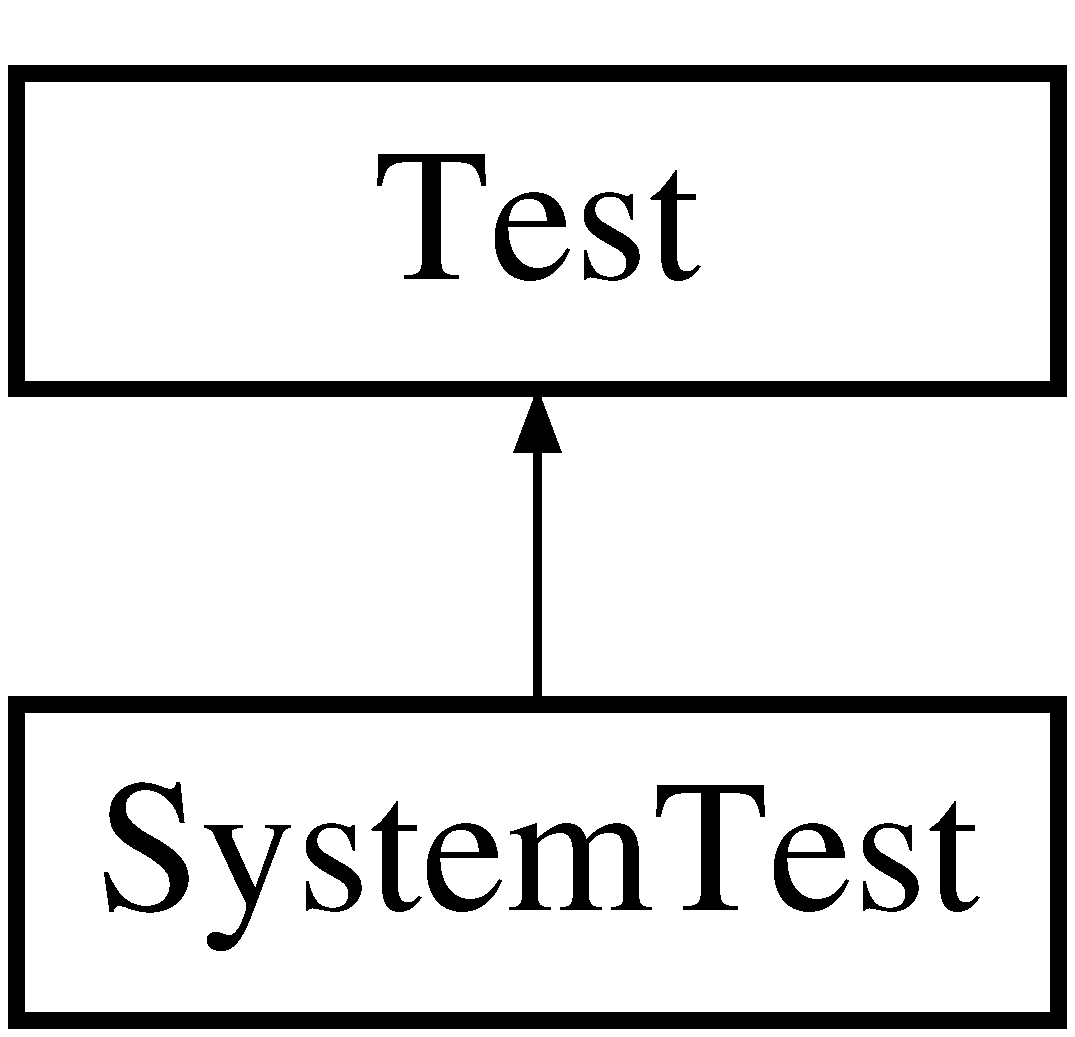
\includegraphics[height=2.000000cm]{class_system_test}
\end{center}
\end{figure}
\subsection*{Protected Member Functions}
\begin{DoxyCompactItemize}
\item 
\hypertarget{class_system_test_a611fccdf6ed757b80f2dda918ed27bc0}{virtual void {\bfseries Set\-Up} ()}\label{class_system_test_a611fccdf6ed757b80f2dda918ed27bc0}

\end{DoxyCompactItemize}
\subsection*{Protected Attributes}
\begin{DoxyCompactItemize}
\item 
\hypertarget{class_system_test_a5655f7f306ac99a2defe7504b593886c}{\hyperlink{classsystem_definition}{system\-Definition} {\bfseries a}}\label{class_system_test_a5655f7f306ac99a2defe7504b593886c}

\item 
\hypertarget{class_system_test_a55d8b8e8bd1ad2755e9a560d1262d57e}{int {\bfseries natoms}}\label{class_system_test_a55d8b8e8bd1ad2755e9a560d1262d57e}

\item 
\hypertarget{class_system_test_a01059fcb317cac6e522903a0f5f24741}{float {\bfseries mass}}\label{class_system_test_a01059fcb317cac6e522903a0f5f24741}

\item 
\hypertarget{class_system_test_a51339a0790891b5b4e2b8689f8bb6b4e}{float {\bfseries L}}\label{class_system_test_a51339a0790891b5b4e2b8689f8bb6b4e}

\item 
\hypertarget{class_system_test_a5ec2ee91805410518f5662b6b41e395b}{float {\bfseries eps}}\label{class_system_test_a5ec2ee91805410518f5662b6b41e395b}

\item 
\hypertarget{class_system_test_a2022b261d402b0617620e0b1745a25bc}{float {\bfseries sigma}}\label{class_system_test_a2022b261d402b0617620e0b1745a25bc}

\item 
\hypertarget{class_system_test_a970b77c65ebefa8d207538700ebdd4a0}{\hyperlink{classnvt___n_h}{nvt\-\_\-\-N\-H} {\bfseries integrate}}\label{class_system_test_a970b77c65ebefa8d207538700ebdd4a0}

\end{DoxyCompactItemize}


\subsection{Detailed Description}


Definition at line 11 of file unittests.\-cpp.



The documentation for this class was generated from the following file\-:\begin{DoxyCompactItemize}
\item 
/\-Users/nathanmahynski/\-C\-B\-E\-M\-D\-G\-P\-U/unittests.\-cpp\end{DoxyCompactItemize}

\addcontentsline{toc}{part}{Index}
\printindex
\end{document}
